\documentclass[12pt]{iopart}
\newcommand{\gguide}{{\it Preparing graphics for IOP journals}}
%Uncomment next line if AMS fonts required
%\usepackage{iopams}  
\usepackage{natbib}
  % this is to disable \equation definition by iop and leave it to asmathet
  \expandafter\let\csname equation*\endcsname\relax
  \expandafter\let\csname endequation*\endcsname\relax
\usepackage{amsmath}
\usepackage{graphics}
\usepackage{graphicx}
\usepackage{caption}
\usepackage{color}
\usepackage{soul}
\usepackage{subfig}
\usepackage{booktabs}
\usepackage{subcaption}
\usepackage{subfigure}
\usepackage{pdfpages}

\usepackage{wrapfig}
%\usepackage{subfig}
\captionsetup[subfigure]{labelformat=empty}



 
\setstcolor{red}
\bibpunct{(}{)}{;}{a}{,}{,}

\usepackage{hyperref}
\hypersetup{
    colorlinks=true,
    linkcolor=blue,
    filecolor=magenta,      
    urlcolor=cyan,
}

\urlstyle{same}

\begin{document}

\title{12-lead ECG classification using Explainable Neural Networks and Ensemble models}

\author{ 
Bjørn-Jostein Singstad$^{1}$%, 
%Tony N Other$^2$ 
%and Bob B Smoot$^3$
\\
\small{
$^1$ Department of Physics, University of Oslo, Oslo, Norway\\
%$^2$ Department of Biomedical Engineering, Georgia Institute of Technology, Atlanta, GA, USA\\
%$^3$ Institute for Medical Engineering \& Science, Massachusetts Institute of Technology, USA\\
}}

\ead{b.j.singstad@fys.uio.no}



%%%%%%%%%%%%%%%%%%%%%%%%%%%%%%%%%%%%%%%%%%%%%%%%%
\begin{abstract}


Existing, commercially available ECG algorithms are mainly rule-based and have limitations in their accuracy. Machine learning, which have shown great performance in many fields over the last years, can possibly outperform the existing ECG-algorithms. This study builds on the Physionet/Computing in Cardiology challenge 2020 which aimed to classify multiple diagnoses based on $43101$ 12-lead ECGs. The models presented are convolutional neural networks and ensemble models based on clustering and random forests. These models are complex and often seen as black boxes in terms of explainability. This study addresses this problem by showning how local interpretable model-agnostic explanations (LIME) can be used to explain the predictions of such models.

The best Ensemble model, utilizing features from all 12 leads, outperformed the convolutional neural networks in this study, with a average cross-validated Physionet/Computing in Cardiology Challenge score of $0.512\pm 0.006$. This score are only $0.021$ behind the cross-validated score, on the same development set, reported by the winner of the Physionet/Computing in Cardiology Challenge 2020.



\end{abstract}


\maketitle


%%%%%%%%%%%%%%%%%%%%%%%%%%%%%%%%%%%%%%%%%%%%%%%%%
\section{Introduction}
Cardiovascular diseases is one of the leading causes of death in the world. Numbers from WHO estimates that $17.9$ million people died from cardiovascular death (CVD) in 2016 which represented $31\%$ of all global death that year \cite{noauthor_cardiovascular_nodate}. Early detection of patient with risk of CVD could potentially decrease the amount of CVD. Electrocardiography is a method with a huge potential for detecting patients with risk of CVD. The electrocardiograph is non-invasive and relativly easy to use, compared to methods like echocardiogram and MRI, which makes it an convenient diagnostic tool. As an example of how widely the electrcardigraph is used, National Ambulatory Medical Care reported that 40 millions electrocardiograms (ECG) were recorded in USA in 2015 \cite{us_department_of_health_and_human_services_national_2015}.

An electrocardiograph measures the electrical activity of the heart from electrodes placed on the surface of the upper body. The result of such a measurement is an ECG. The ECG is a graphical representation of the measured electrical activity of the heart with respect to time. One of the challenges is that the ECG can be difficult to interpret correctly. The interpretation can be time consuming and require a high degree of expertise \cite{bickerton_misplaced_2019}.

Many of the modern and clinically used electrocardiographs today are equipped with a built-in interpretation program. The interpretation program analyzes the ECG and prints interpretive texts that may indicate different diseases. Studies show that there are some limitations to the automatic interpretation algorithms \cite{schlapfer_computer-interpreted_2017, smulyan_computerized_2019}. The errors, caused by the automatic interpretation algorithms, means that doctors or cardiologists has to read over the ECGs to ensure they are correct.

The hypothesis in this study is that machine learning can improve today's interpretive algorithms. Eight machine learning models from a previous study \cite{singstad_convolutional_nodate} will be evaluated and compared with two new machine learning models, were one of them will utilize 12 lead and the other will utilize only 2 leads. 

A considerable amount of literature has been published on heartbeat classification \cite{annam_classification_2020}, single \cite{mathews_novel_2018} and even  2-lead classifiaction \cite{liu_arrhythmia_2013} over the last ten years . In most recent years there have been an increasing focus on 12-lead ECG classificaion and some recent studies has shown that machine learning is feasible \cite{ribeiro_automatic_2020, yao_multi-class_2020,li_automatic_2020, chen_detection_2020}. On the other hand, the  dataset used has either been small and homogeneous \cite{noauthor_classification_nodate} or not accessible to everyone. In this study, a large, open dataset from several sources and a large variation in different diagnoses will be examined and used as development set for training machine learning models \cite{alday_classification_2020}. This dataset was used in a challenged held by PhysioNet \cite{goldberger_physiobank_2000} and Computing in Cardiology (CinC) in 2020 were $217$ teams submitted $1395$ algorithms during the challenge \cite{alday_classification_2020}. A training set and a test set were provided and the team who got the best score on the test set won the competition. The best team called themselves \textit{prna} and they achieved a PhysioNet/CinC Challenge score \cite{alday_classification_2020} of $0.533$ on the test set and a cross-validated score of $0.533\pm 0.046$ (mean and standard deviation). 

It is already stated that PhysioNet/CinC Challenge 2021 will utilize the same dataset, but this time investigate both 12-lead and 2-lead ECG in a challenge called "will 2 to?". One of the objective of this study is to prepare an initial submission to the PhysioNet/CinC Challenge 2021 which will go live in the end of December 2020.

In addition, this study will demonstrate how to get an explainable prediction from the machine learning models developed in this study. Explainability of machine learning models is a new field in artificial intelligence (AI) and is called explainable AI. Explainable predictions are very important in medical diagnostics. As an example, cardiologists and doctors can use their knowledge to see if the parameters used for the prediction, by an ECG classification model, can be explained physiologically. This will probably lead to better trustworthiness for an ECG classification algorithm among cardiologists and doctors.

%\section{Background}
%\subsection{Explainable AI}
In addition, Article 22 of GDPR, in essence, grants an individual a “right of human intervention.” Under this right, an individual may ask for a human to review the AI’s decision to determine whether or not the system made a mistake. This right of human intervention and the right of explainability together place a legal obligation on the business to understand what happened, and then make a reasoned judgment as to if a mistake was made.[https://www.airoboticslaw.com/blog/ai-explainability-gdpr]

\section{Methods}
\subsection{Data}
The PhysioNet/CinC Challenge 2020 development set consisted of $43101$ ECG-recordings. The datasets were sourced from six subset from four different sources:

\begin{itemize}
    \item The first source is China Physiological Signal Challenge 2018 wich consists of two subsets: The original China Physiological Signal Challenge 2018 dataset \cite{liu_open_2018} and a extra set called China Physiological Signal Challenge Extra. 
    \item The second source is the Physikalisch-Technische Bundesanstalt (PTB) which consist of two subsets. The first one is the PTB Diagnostic \cite{bousseljot_nutzung_2009} and the second subset is PTB-XL \cite{wagner_ptb-xl_2020-1}
    \item The third source is the St. Petersburg Institute of Cardiological Technics (INCART) database \cite{goldberger_physiobank_2000}
    \item  The fourth is the Georgia 12-Lead ECG Challenge Database which is new database and is still not described in any paper other than the PhysioNet/CinC Challenge 2020 paper \cite{alday_classification_2020}.
\end{itemize}
A total of $111$ different diagnoses were present in the total dataset. Each ECG-recording had at least one diagnosis, but some also had more than one diagnosis. The classification of such a data set is considered a multi-label, multi-class classification problem. The goal of PhysioNet / CinC Challenge 2020 was to classify $27$ of the $111$ diagnoses. 



\subsubsection{Splitting of data}

The data were splitted into training (90\%) and validation (10\%) data using 10-fold stratified cross-validation with random state $=42$ \cite{pedregosa_scikit-learn_2011}. The stratification arranged the splitting such that the distribution of diagnoses was the same in both the train and validation data.

\subsection{Preprocessing data}
Initially the diagnosis were encoded with Systematized Nomenclature of Medicine Clinical Terms (SNOMED-CT). The SNOMED-CT codes were decoded into human readable diagnosis and one-hot encoded into a $27$-bit long array. Each of the bits in the array represented one of the $27$ scored diagnosis in the PhysioNet/CinC Challenge 2020 \cite{alday_classification_2020}. The $84$ unscored diagnoses were overlooked and did not represent any change in the 27-bit long label array. The same labels were used in both the CNN-models and the ensemble models, the preprocessing and feature extraction from the ECG were done differently for the CNN model and for the ensemble model.

\subsubsection{Preprocessing for Convolutional models} \hfill \break
All ECG-recordings used by the CNN-models were padded or truncated to a signal length of $5000$ samples. Padding and truncation were done by removing any parts longer than $5000$ samples and adding a tail of $5000 - n$ zeros to any recording of length $n<5000$. The rule-based model on the other hand, which was used in two of eight CNN-models, analyzed the ECG before padding or truncation to $5000$ samples.

The $27$ diagnoses/classes were not balanced and, to prevent the CNN-models to learn more from the diagnosis that occur more frequently in the dataset, a class weight were calculated. The weights were fed to the models during training and gave higher priority to ECGs with rare diagnosis than diagnosis that occur more frequently in the dataset. 

\subsubsection{Preprocessing for the ensemble models}\hfill \break
All ECG recordings were fed into a ECG-featurizer function \cite{bjorn-jostein_singstad_ecg-featurizer_nodate}. The ECG-Featurizer analyzed the ECGs and extracted $112$ features from the ECGs. All of the $112$ features were used in the 12-lead classification while only $63$ were used in the 2-lead classification. Only features that were extracted from lead $II$ and V5 were used in the 2-lead model.

$42 720$ of $43101$ ECGs were successfully featurized på the ECG-featurizer. In addition, $146$ ECG-recordings were removed due to missing values. This gave a total dataset of $42574$ succesfully featurized ECGs to use by the ensemble model.


\subsection{Model architectures}
\subsubsection{CNN architectures}\hfill \break
The CNN architectures used in this study was the same as in \cite{bjorn-jostein_singstad_classifying_2020}. The models are listed in table \ref{tab:modelcombo}. The new contribution in this study is that the $8$ models were scored using cross-validation on the development data. \newline\newline

\vspace{4 mm}
\begin{table}[!htb]
        \centering
        \caption{The eight CNN models developed in \cite{bjorn-jostein_singstad_classifying_2020} and used in this study}
            \scalebox{1.0}{
                \begin{tabular}{lr} \hline\hline
                        Model     \\\hline
                        A) FCN                       \\
                        B) Encoder                   \\
                        C) FCN $||$ age, gender              \\   
                        D) Encoder $||$ age, gender       \\
                        E) Encoder $||$ FCN            \\
                        F) Ecoder $||$ FCN $||$ age, gender     \\
                        G) Encoder $||$ FCN + rule-based model      \\
                        H) Encoder $||$ FCN $||$ age, gender + rule-based model    \\\hline\hline
                \end{tabular}}
                \label{tab:modelcombo}
\end{table}
\vspace{4 mm}
\newline

\subsubsection{Ensemble model architecture}\hfill \break
The architectures trained on the featurized ECG-data were build up using scikit-multilearn \cite{szymanski_scikit-multilearn_2019}. Scikit-multilearn is a library for multi-label classification. The ensemble models built using Label Space Partitioning Classifier \cite{szymanski_how_2016}, Classifier Chain \cite{read_classifier_2009} and random forests. Label Space Partitioning Classifier is a cluster algorithm were each cluster is a separate classification problem. The clusters were selected using a method called fixed label space clusterer. This method lets the developer define the clusters. The clusters in this study were created by iterating over all diagnosis in the training set and for the $n$-th diagnosis there was $m_n$ diagnosis that co-existed with the $n$-th diagnosis across the data set. In total there was $27$ clusters and the size of the clusters, $m_n + 1$, were different for each of the folds in the 10-folded cross-validation. This is illustrated in figure \ref{fig:diagnosis_co_exist}.

\begin{figure}[!hbp]
    \centering
    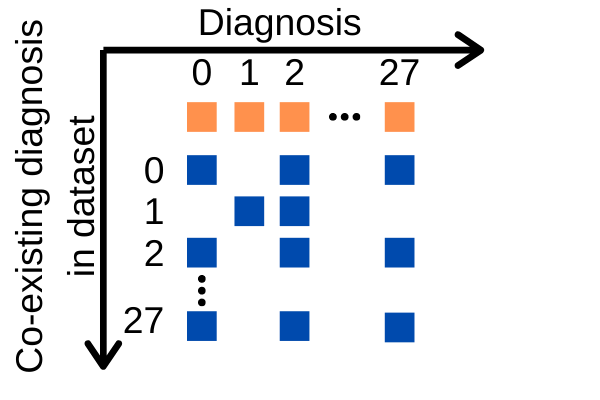
\includegraphics[width=.6\textwidth]{Figures/Diagnosis_cluster_axis.png}
    \caption{The figure shows how each of the 27 diagnosis co-existed with one or more of the other 26 diagnosis when looking across the whole development dataset. The 27 clusters that was used for the ensemble models used the same index as the co-existing diagnosis.}
    \label{fig:diagnosis_co_exist}
\end{figure}



\subsection{Threshold optimization}
For the CNN-models a threshold for the 27 classes had to be set. New thresholds were set for each fold. A method called Nelder-Mead downhill simplex method \cite{nelder_simplex_1965, virtanen_scipy_2020} was used to optimize the thresholds individually with PhysioNet/CinC Challenge score as the optimization goal. This method can be computational heavy and therefore a subset of the training set were used to optimize the threshold. The subset were determined using a stratified 10-fold and then selecting the first validation fold as the threshold optimization set.

The Nelder-Mead downhill simplex method is used to find the local minimum of a function using the function itself and an initial guess of the optimal variable of the function. In the first fold of the 10-folded cross-validation the initial guess for the Nelder-Mead optimization algorithm was found by giving a 27-element long array values of 1 and multiplied it with a variable that was given values from 0 to 1, with a step size of 0.05. The next folds in In the 10-folded cross-validation used the threshold found by the Nelder-Mead in the previos fold as the initial guess. 

The Ensemble models on the other hand did not need any threshold optimiztion as the output were binarized by the model.





\subsection{Explanation models}
To add explainability to the models used in this study a local interpretable model-agnostic explanation (LIME) was used \cite{lime}. LIME explains the feature importance locally for a given prediction. LIME uses a linear model to explain the prediction of the the mode complex CNNs and ensemble models used in this study. As a proof-of-concept for such explaination models the 12-lead ensemble model and the CNN encoder model were selected to be explained. The ensemble model were explained using a tabular explainer-function.

To explain the CNN model a explainer called recurrent explainer was used. The Encoder model were simplified by swaping the last layer in the Encoder-model with a softmax-layer with two nodes and the dataset were modified such that Normal Sinus Rhythm were equal to Normal class and all other diagnosis were equal to Abnormal class.

\newpage



\section{Results}
\subsection{Cross-validated results}
The CNN models were trained using ADAM-optimizer, a batchsize $30$ and the Area Under the Curve (AUC)-score, on the validation set, was used to reduce learning rate during training. The learning rate was initially at $0.001$ for all models and decreased by a factor of 10, each epoch that the AUC score did not improve. Early stopping used to stop training when AUC score, on the validation data, did not improve over two successive epochs.

The ensemble models were trained using n\_estimators $=$ 3 for the random forest classifier and the input features where scaled using a Standard Scaler \cite{pedregosa_scikit-learn_2011}.

All models were scored using F1, F2, G2 and PhysioNet CinC Challenge score for each of the 10-folds \footnote{All codes and models are available here: \url{https://github.com/Bsingstad/FYS-STK4155-oblig3}}. The results in figure \ref{fig:crossval_score} shows that the random forest-based model, using features from all 12 leads, outperformed the other model on all metrics used in this study. 



\newpage
\begin{figure}[ht!]
\vspace{0em}
  \subfloat[(a) F1-score]{
	\begin{minipage}[c][1\width]{
	   0.5\textwidth}
	   \centering
	   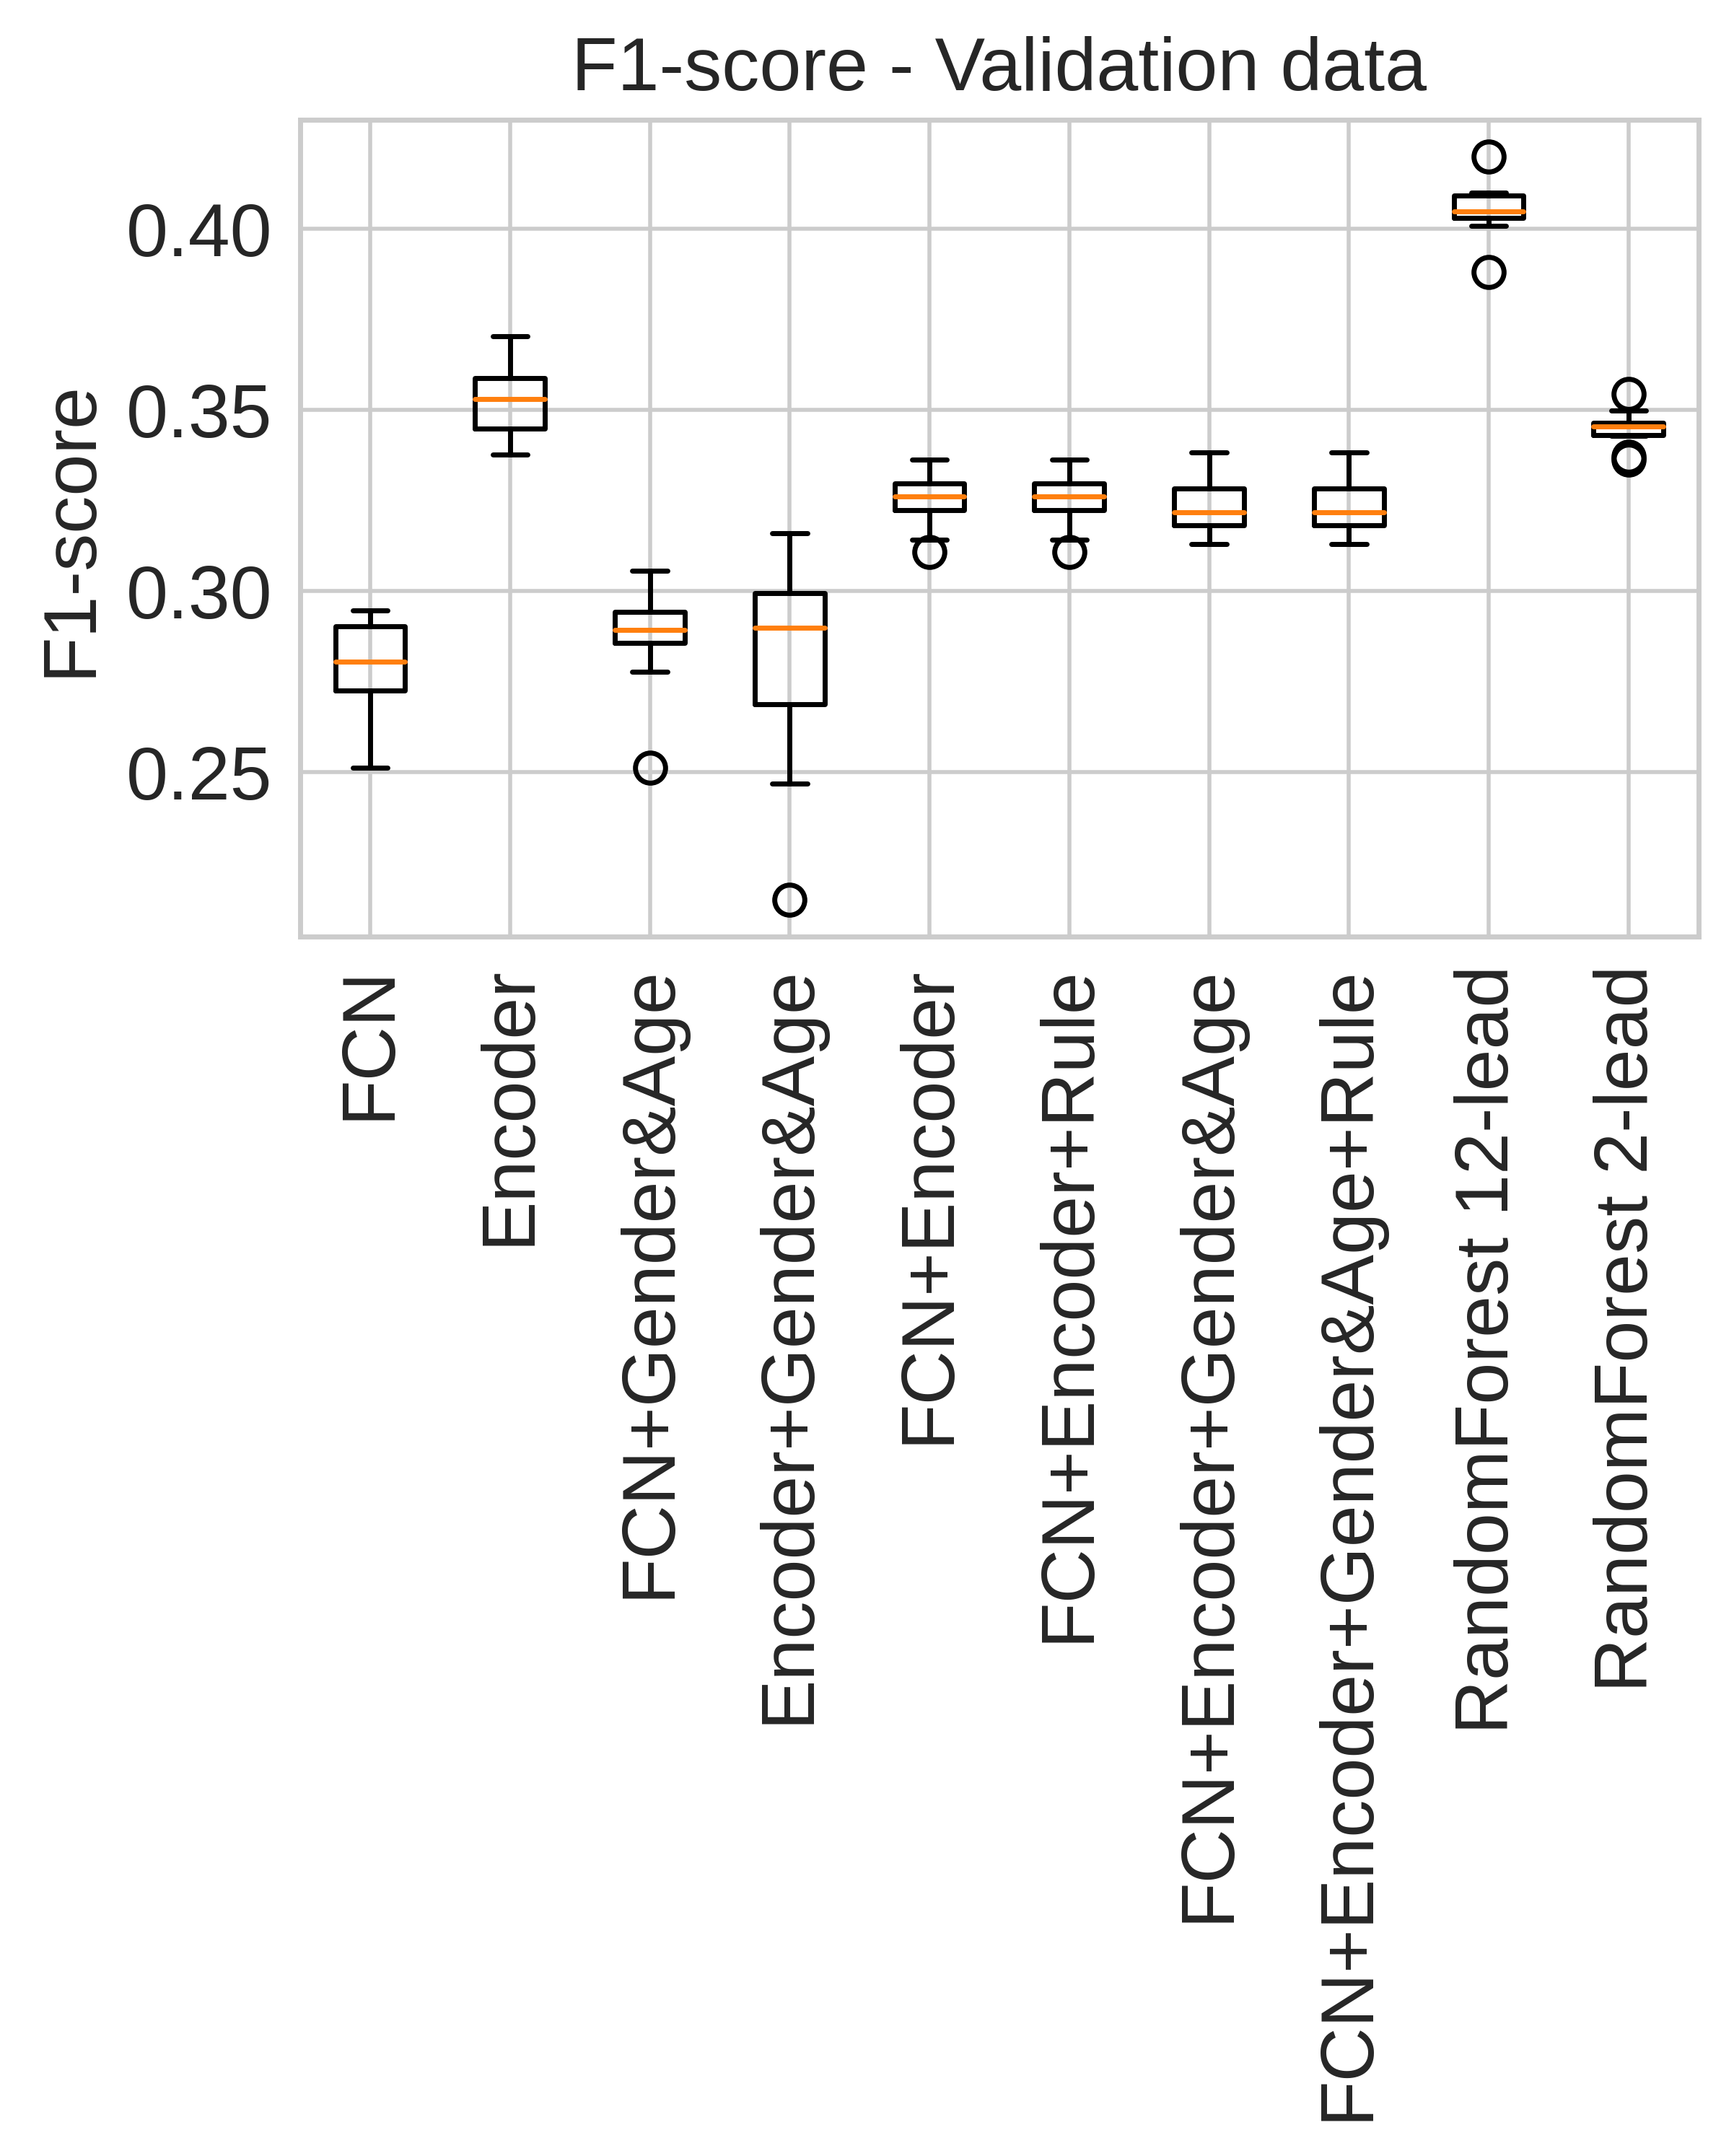
\includegraphics[width=0.9\textwidth]{Figures/F_score_val}
	   \vspace{0em}
	\end{minipage}}
 \hfill 	
  \subfloat[(b) F2-score]{
	\begin{minipage}[c][1\width]{
	   0.5\textwidth}
	   \centering
	   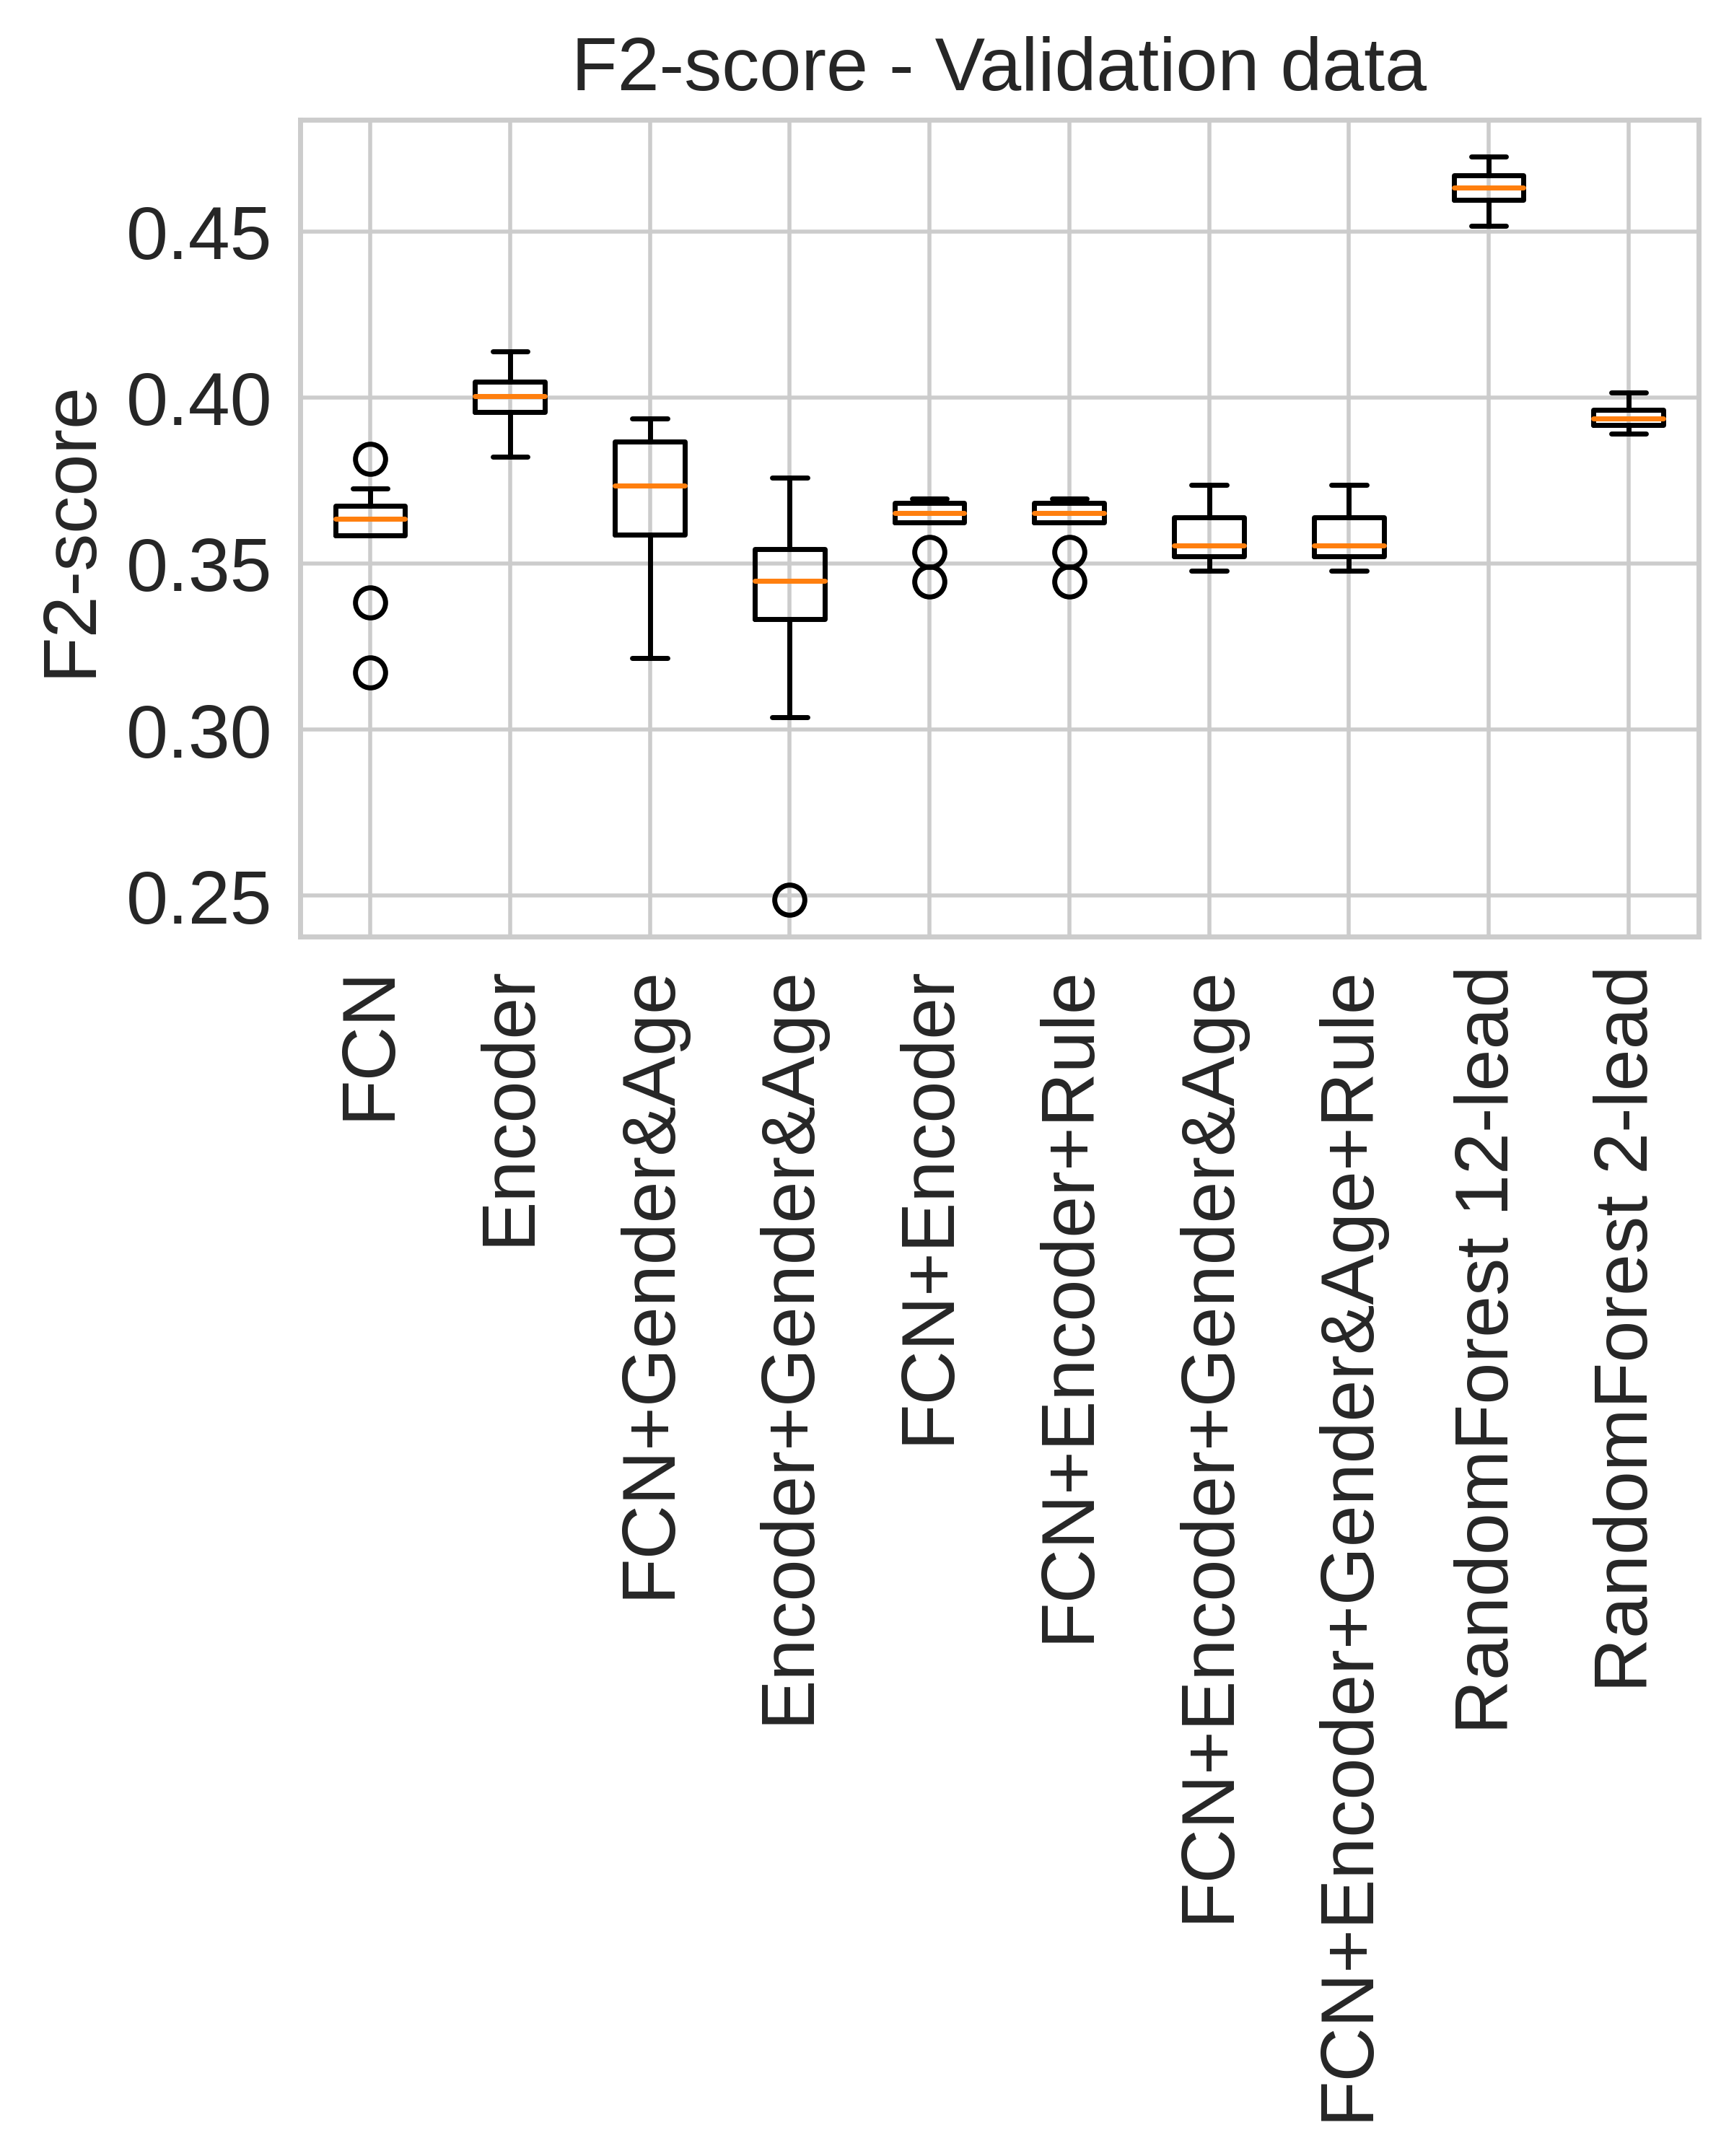
\includegraphics[width=0.9\textwidth]{Figures/F2_score_val}
	   \vspace{0em}
	\end{minipage}}
\end{figure}

\begin{figure}[hb!]
\vspace{0em}
  \subfloat[(c) G2-score]{
	\begin{minipage}[c][1\width]{
	   0.5\textwidth}
	   \centering
	   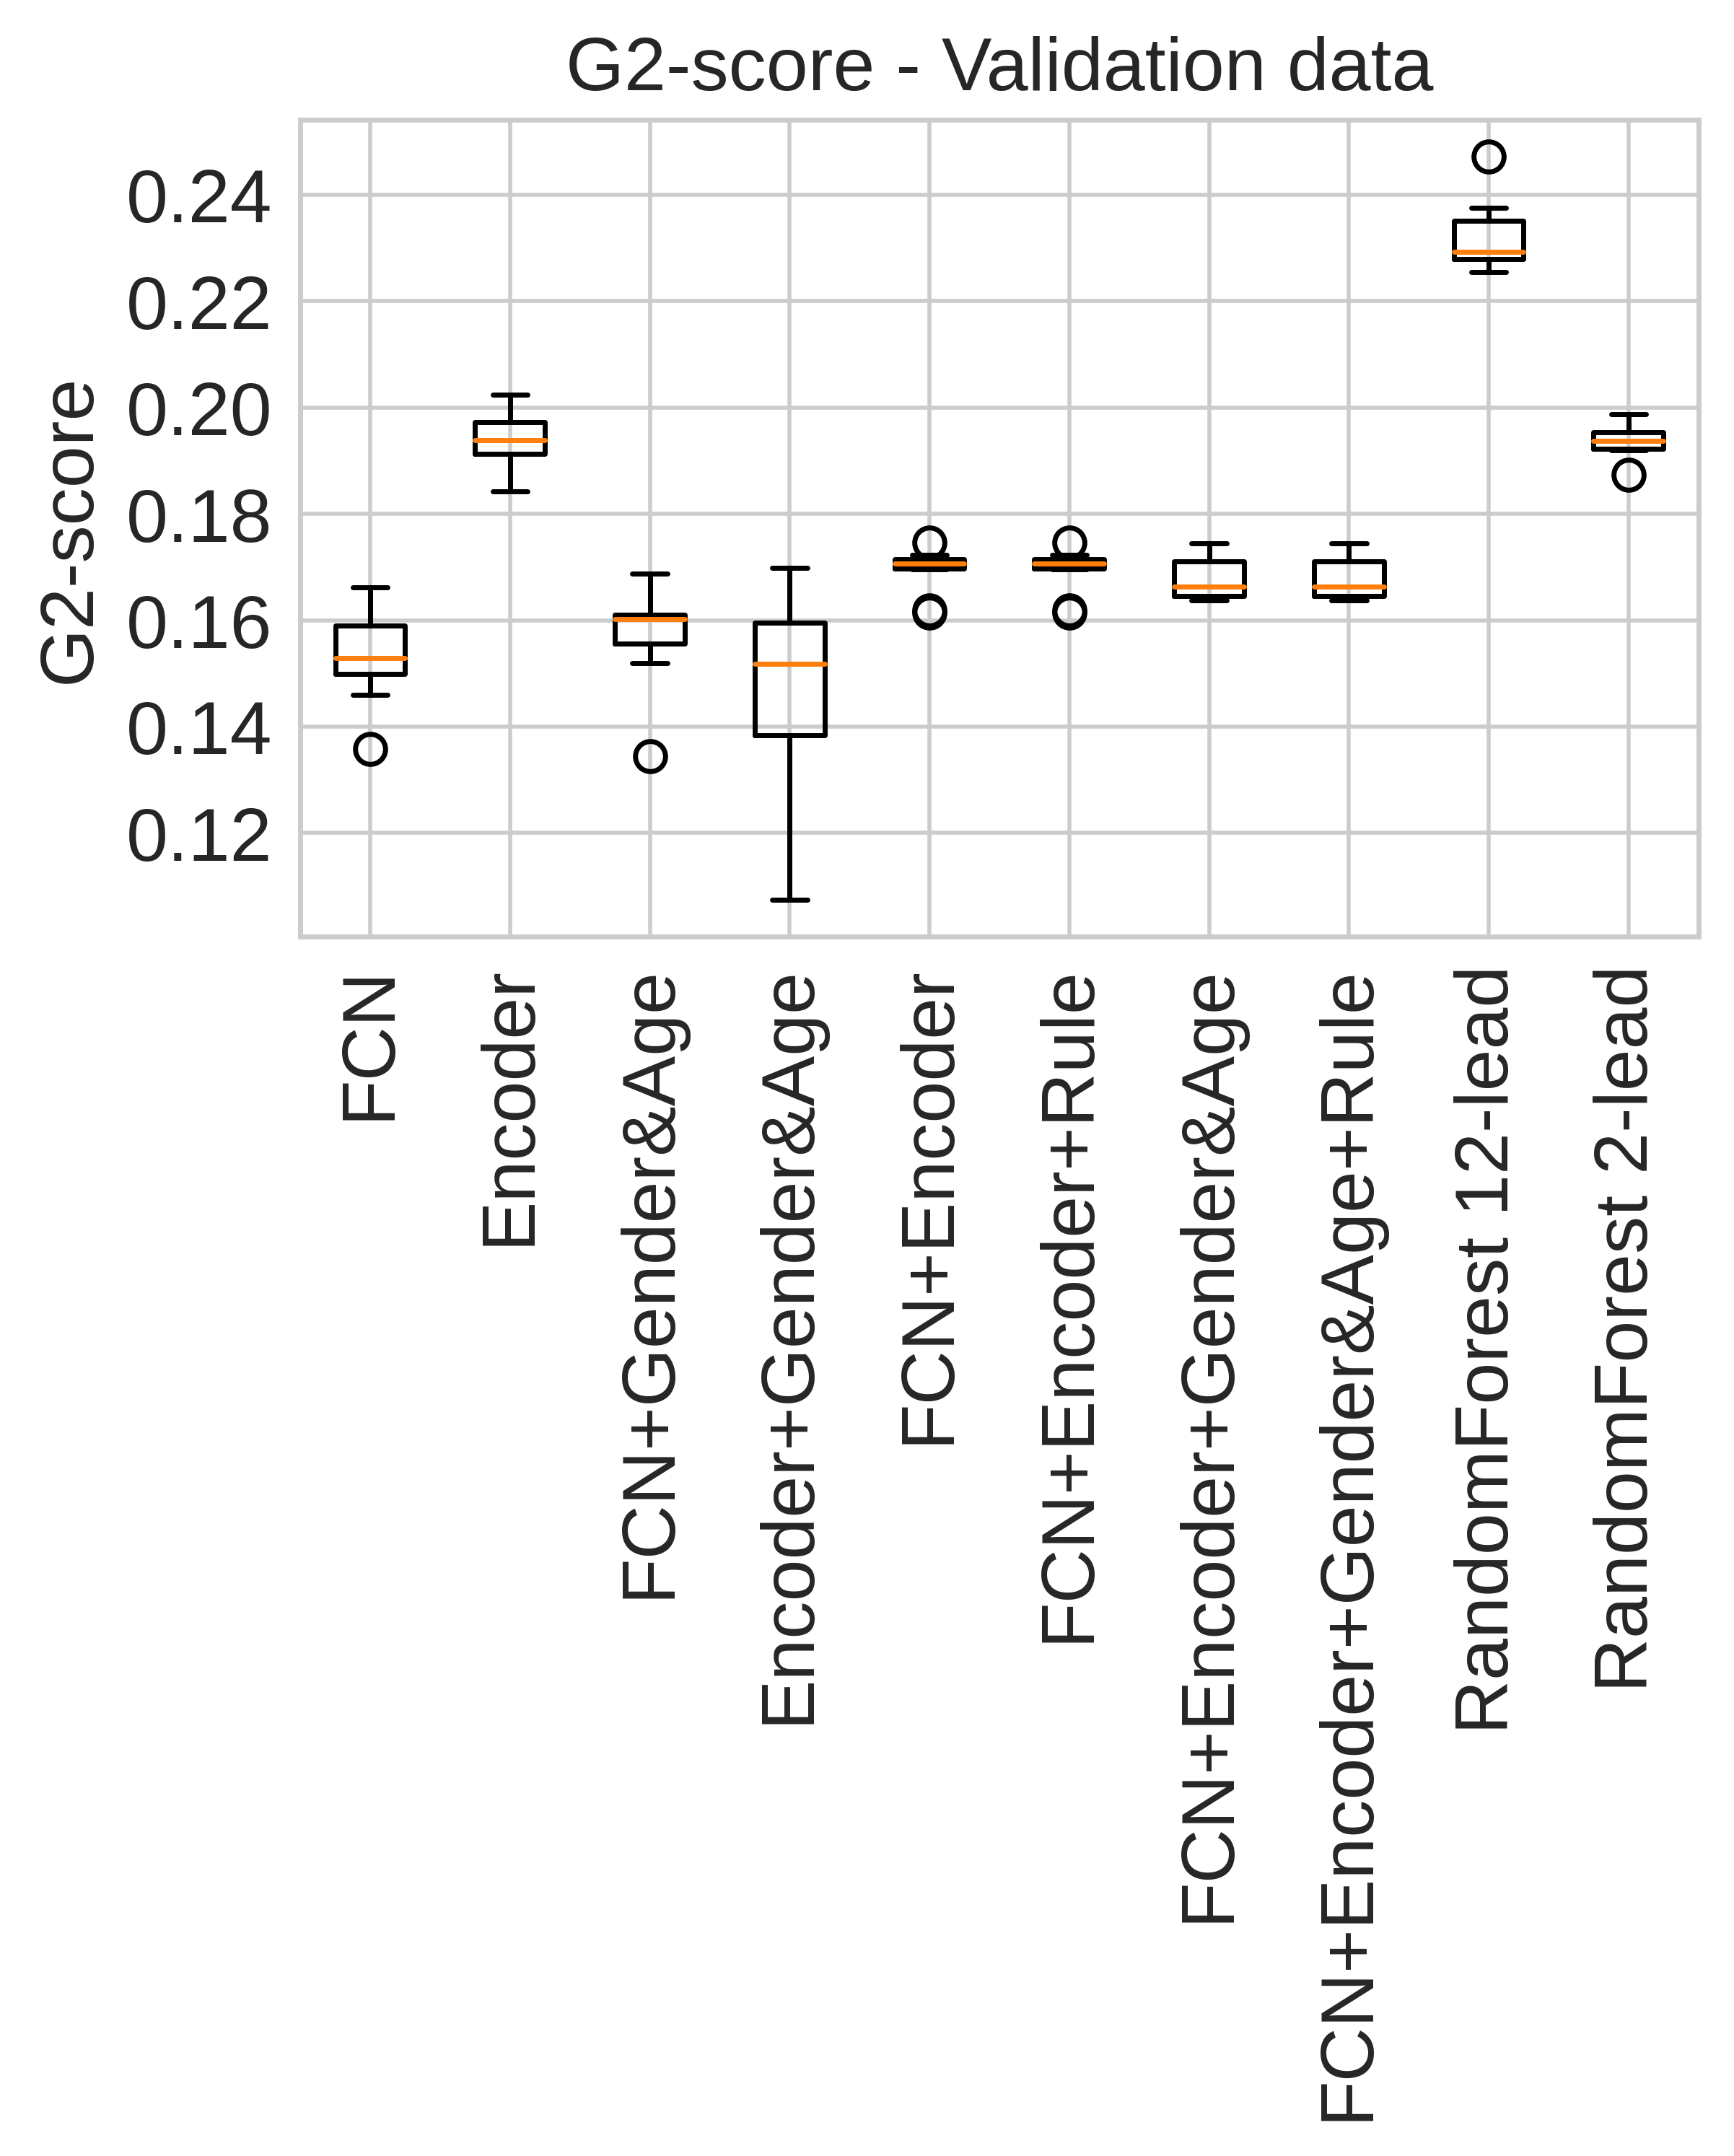
\includegraphics[width=0.9\textwidth]{Figures/G2_score_val}
	   \vspace{1em}
	\end{minipage}}
 \hfill 	
  \subfloat[(d) PhysioNet/CinC Challenge-score]{
	\begin{minipage}[c][1\width]{
	   0.5\textwidth}
	   \centering
	   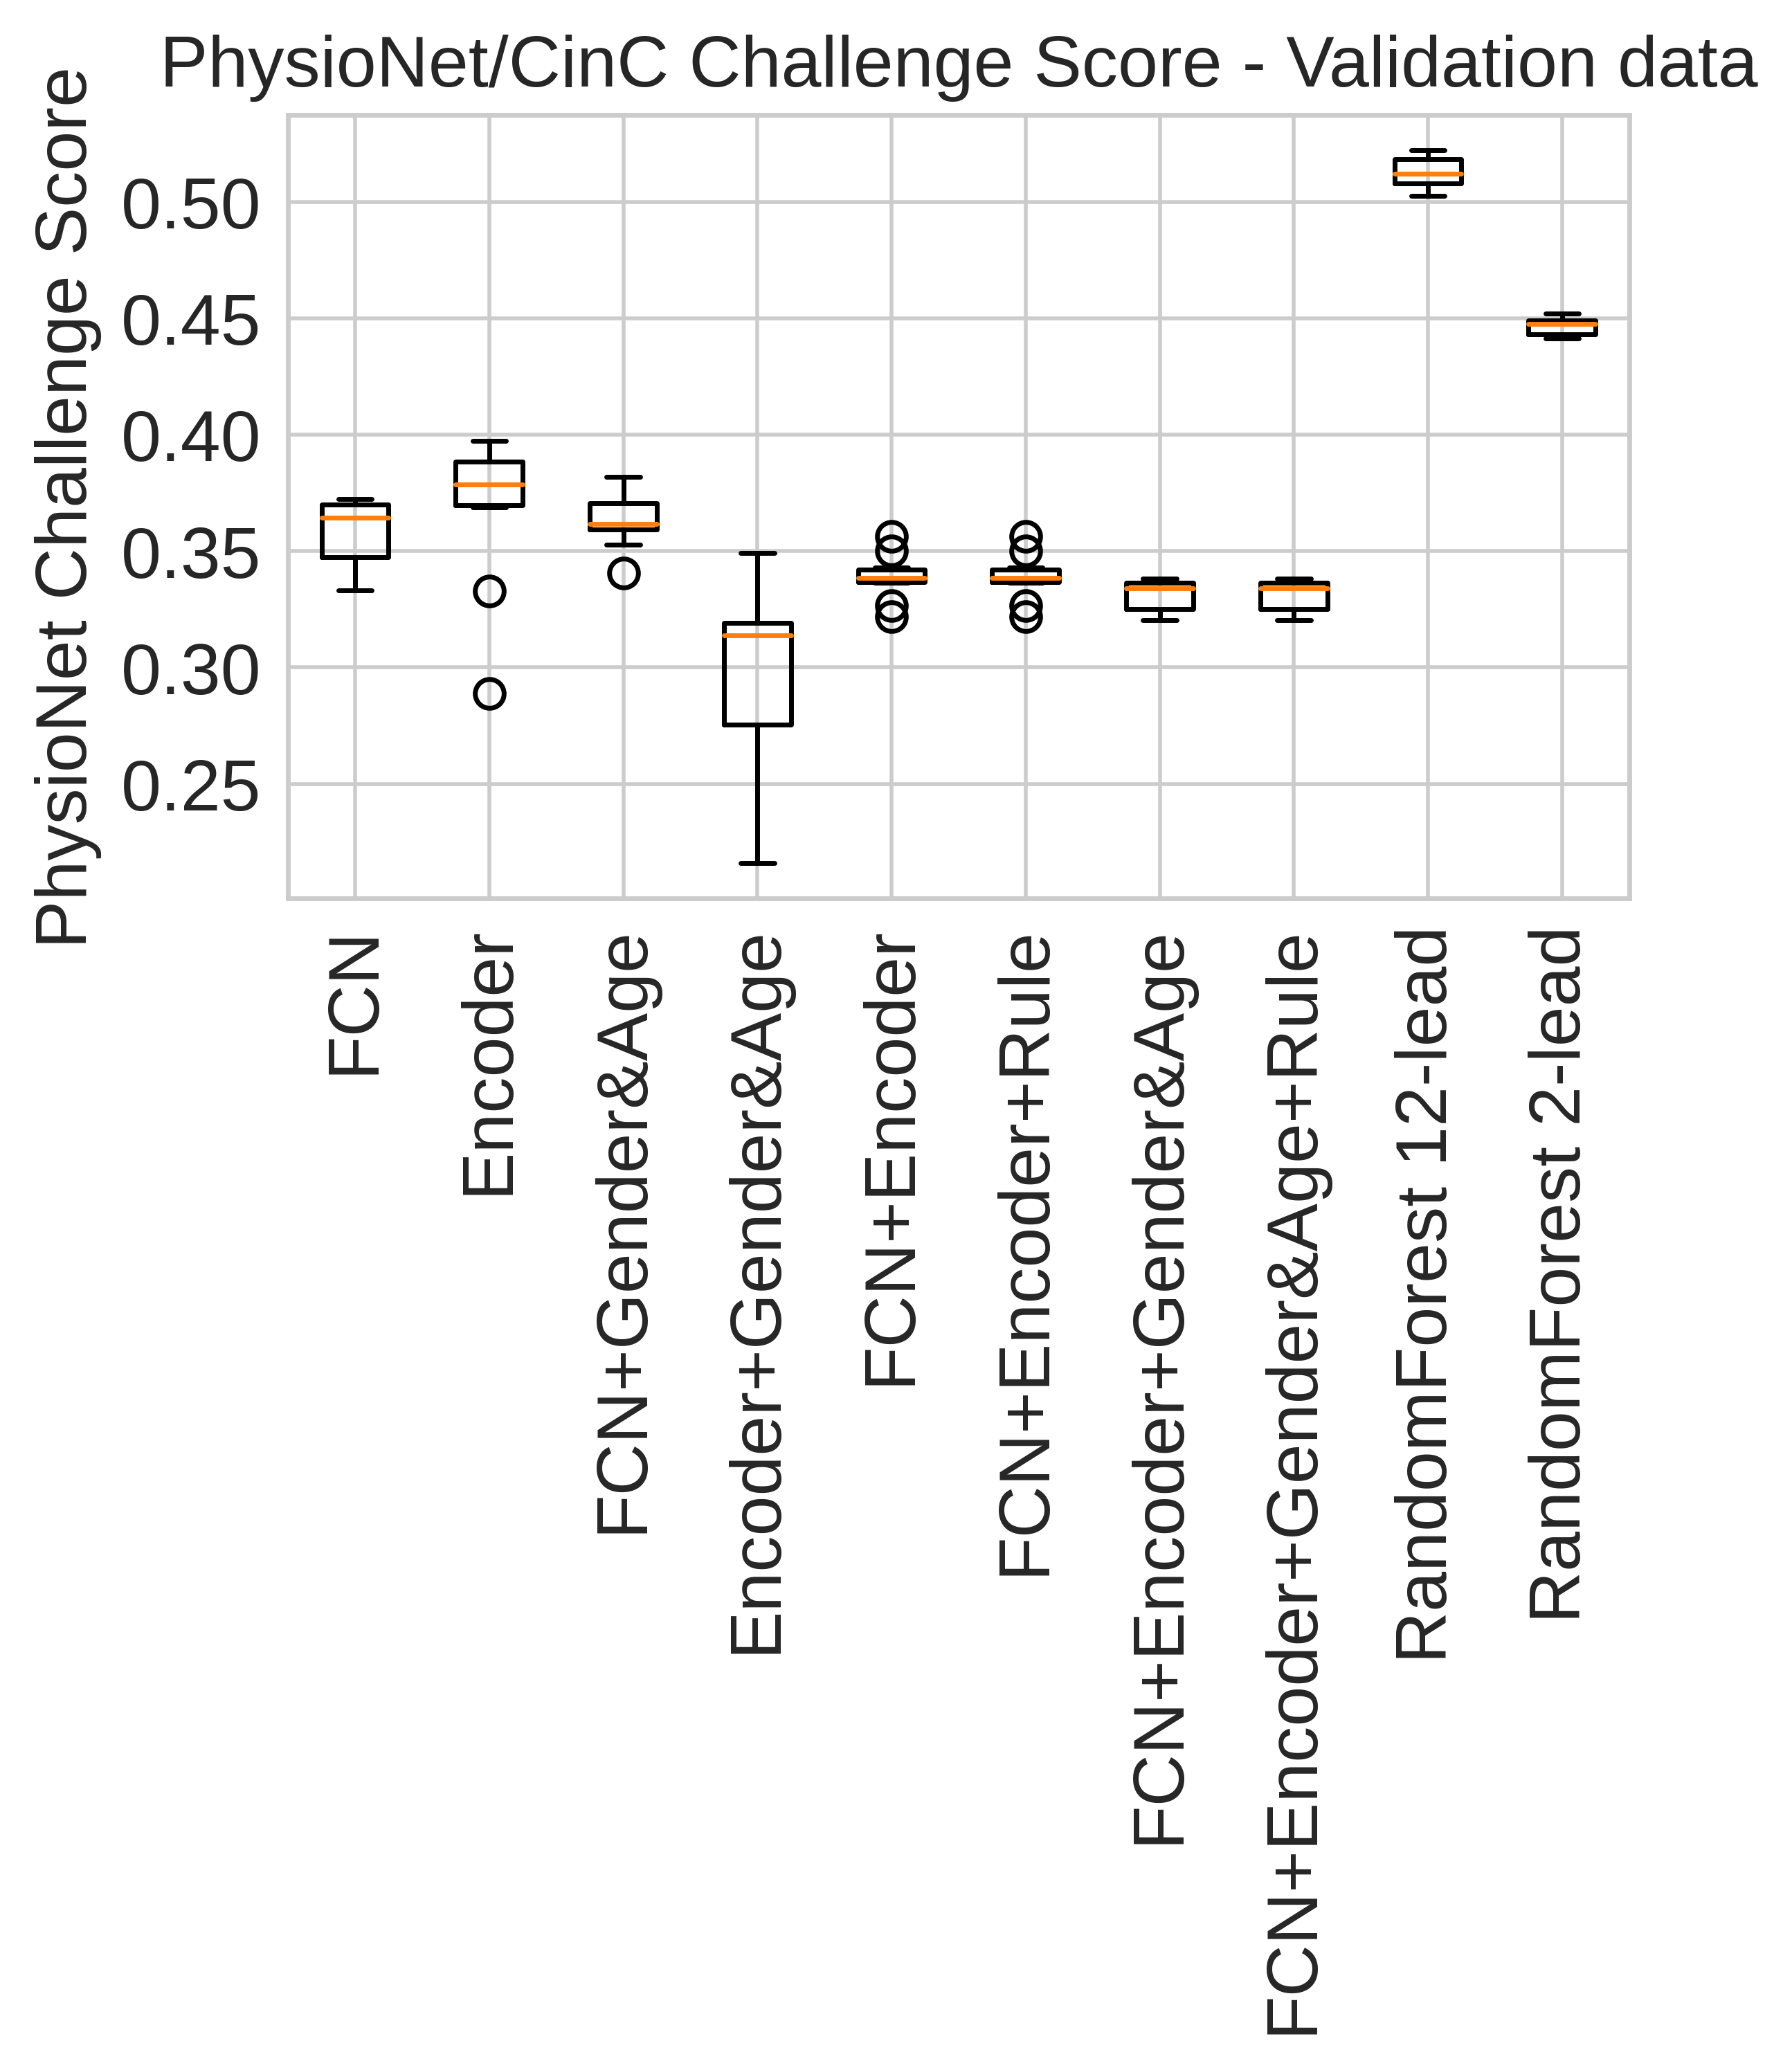
\includegraphics[width=0.9\textwidth]{Figures/PhysioNetChallenge_score_val}
	   \vspace{0em}
	\end{minipage}}
    \caption{The figure shows 10-fold cross-validated scores achieved by ten different models. The upper left show F1-score, the upper right show F2-score, the lower left show G2-score and the lower right show PhysioNet/CinC Challenge score. The PhysioNet/CinC Challenge score are described in \cite{alday_classification_2020}}
\label{fig:crossval_score}
\end{figure}



\subsection{Explainability results}
The tabular explainer that was applied on the ensemble model was trained on $5000$ ECGs from the training data and then tested on a ECG from the test data. The ECG that were explained by the model explainer were from a patient with non-specific intra ventricular conduction disorder (NSIVCB). The explaination is visualized in figure \ref{fig:explainability_rand_12}.

%\begin{figure}[!bp]
%    \centering
%    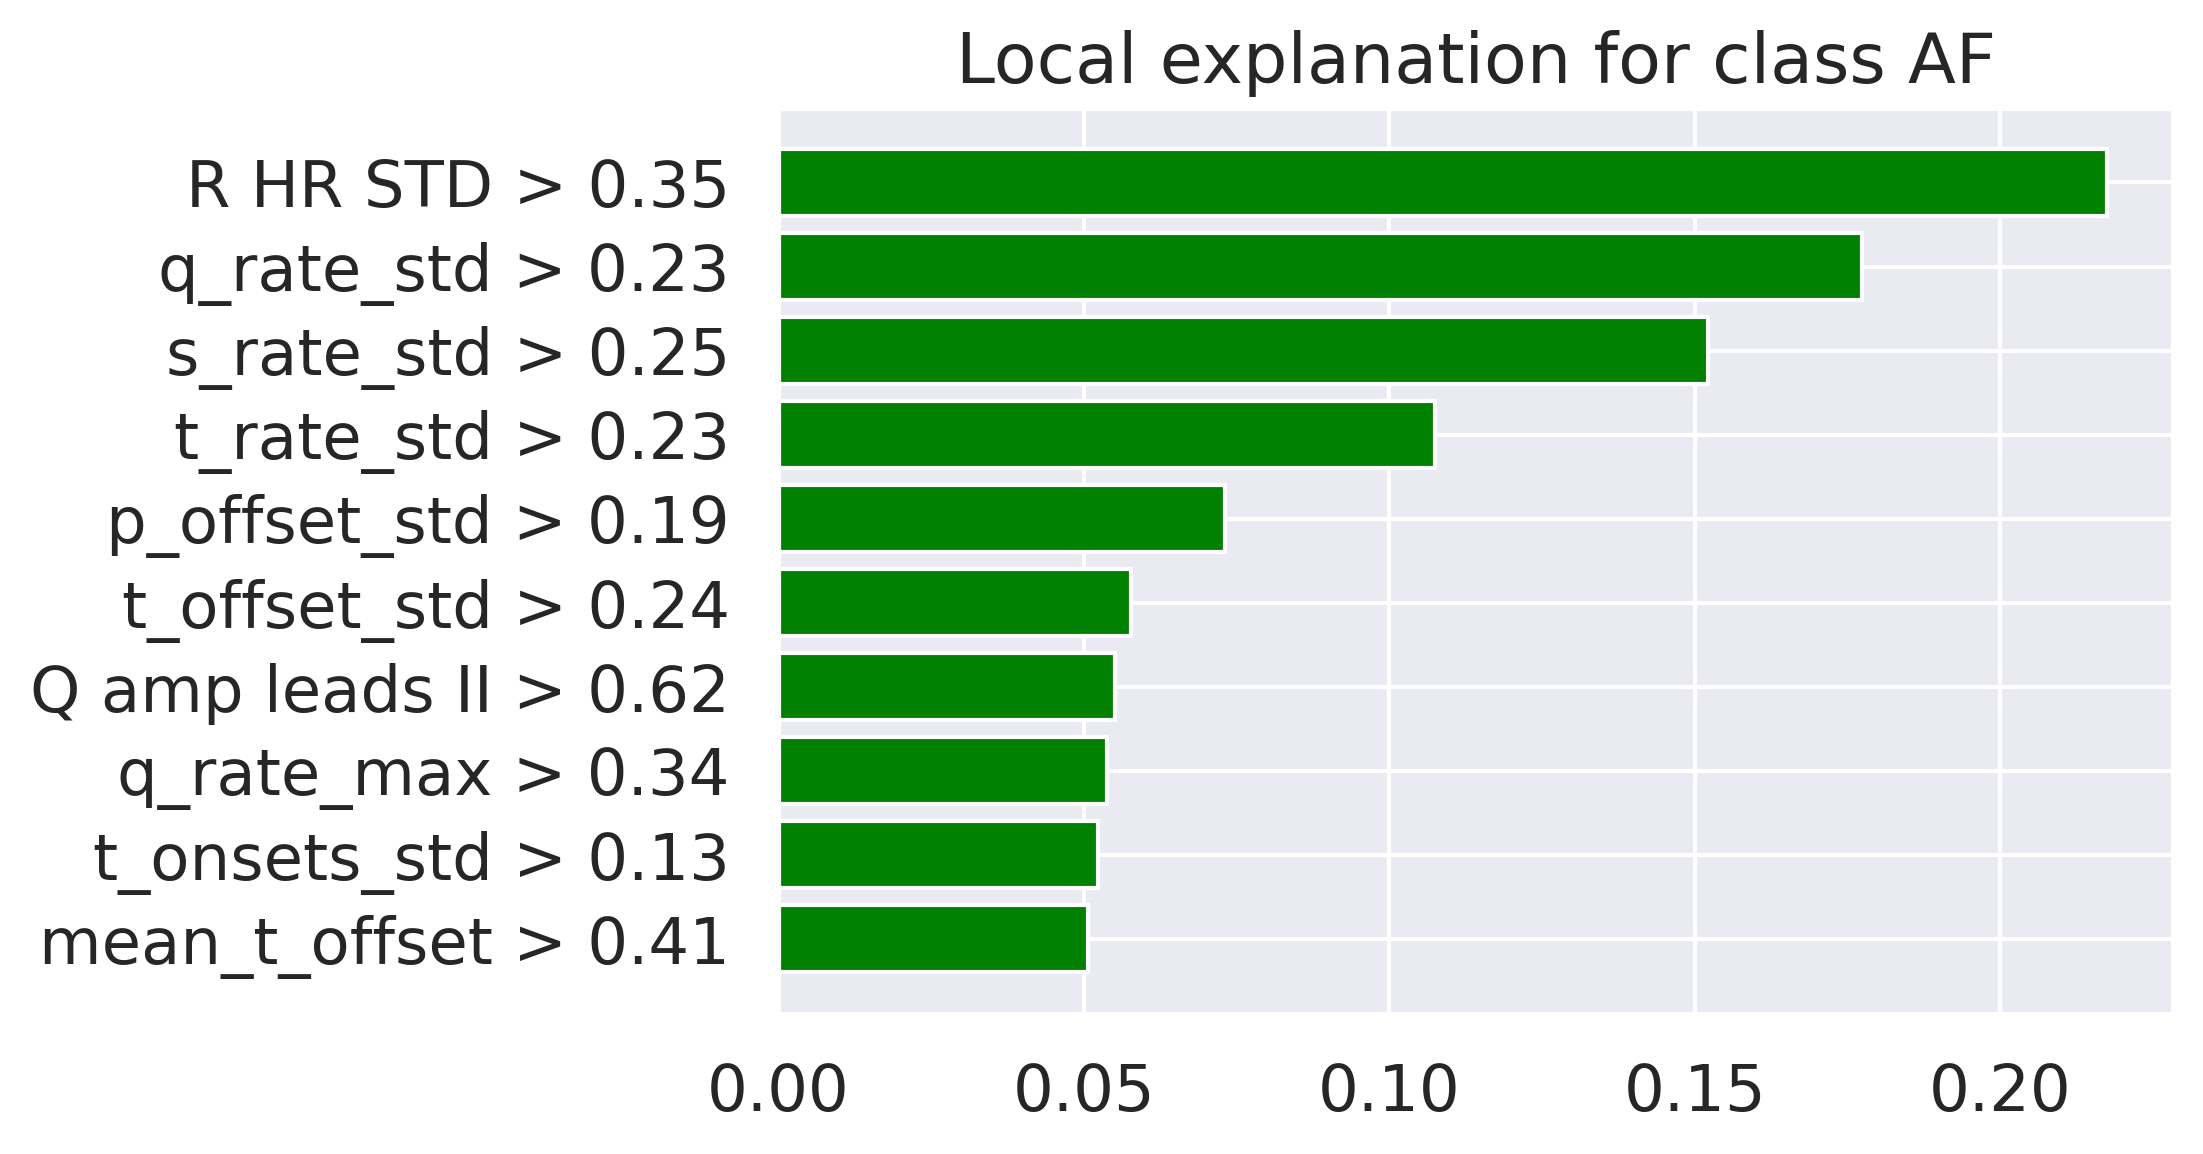
\includegraphics[width=0.8\textwidth]{Figures/atrialfib_atrialfib.png}
%    \caption{}
%    \label{fig:parameterregel}
%\end{figure}
\begin{figure}[!htp]
    \centering
    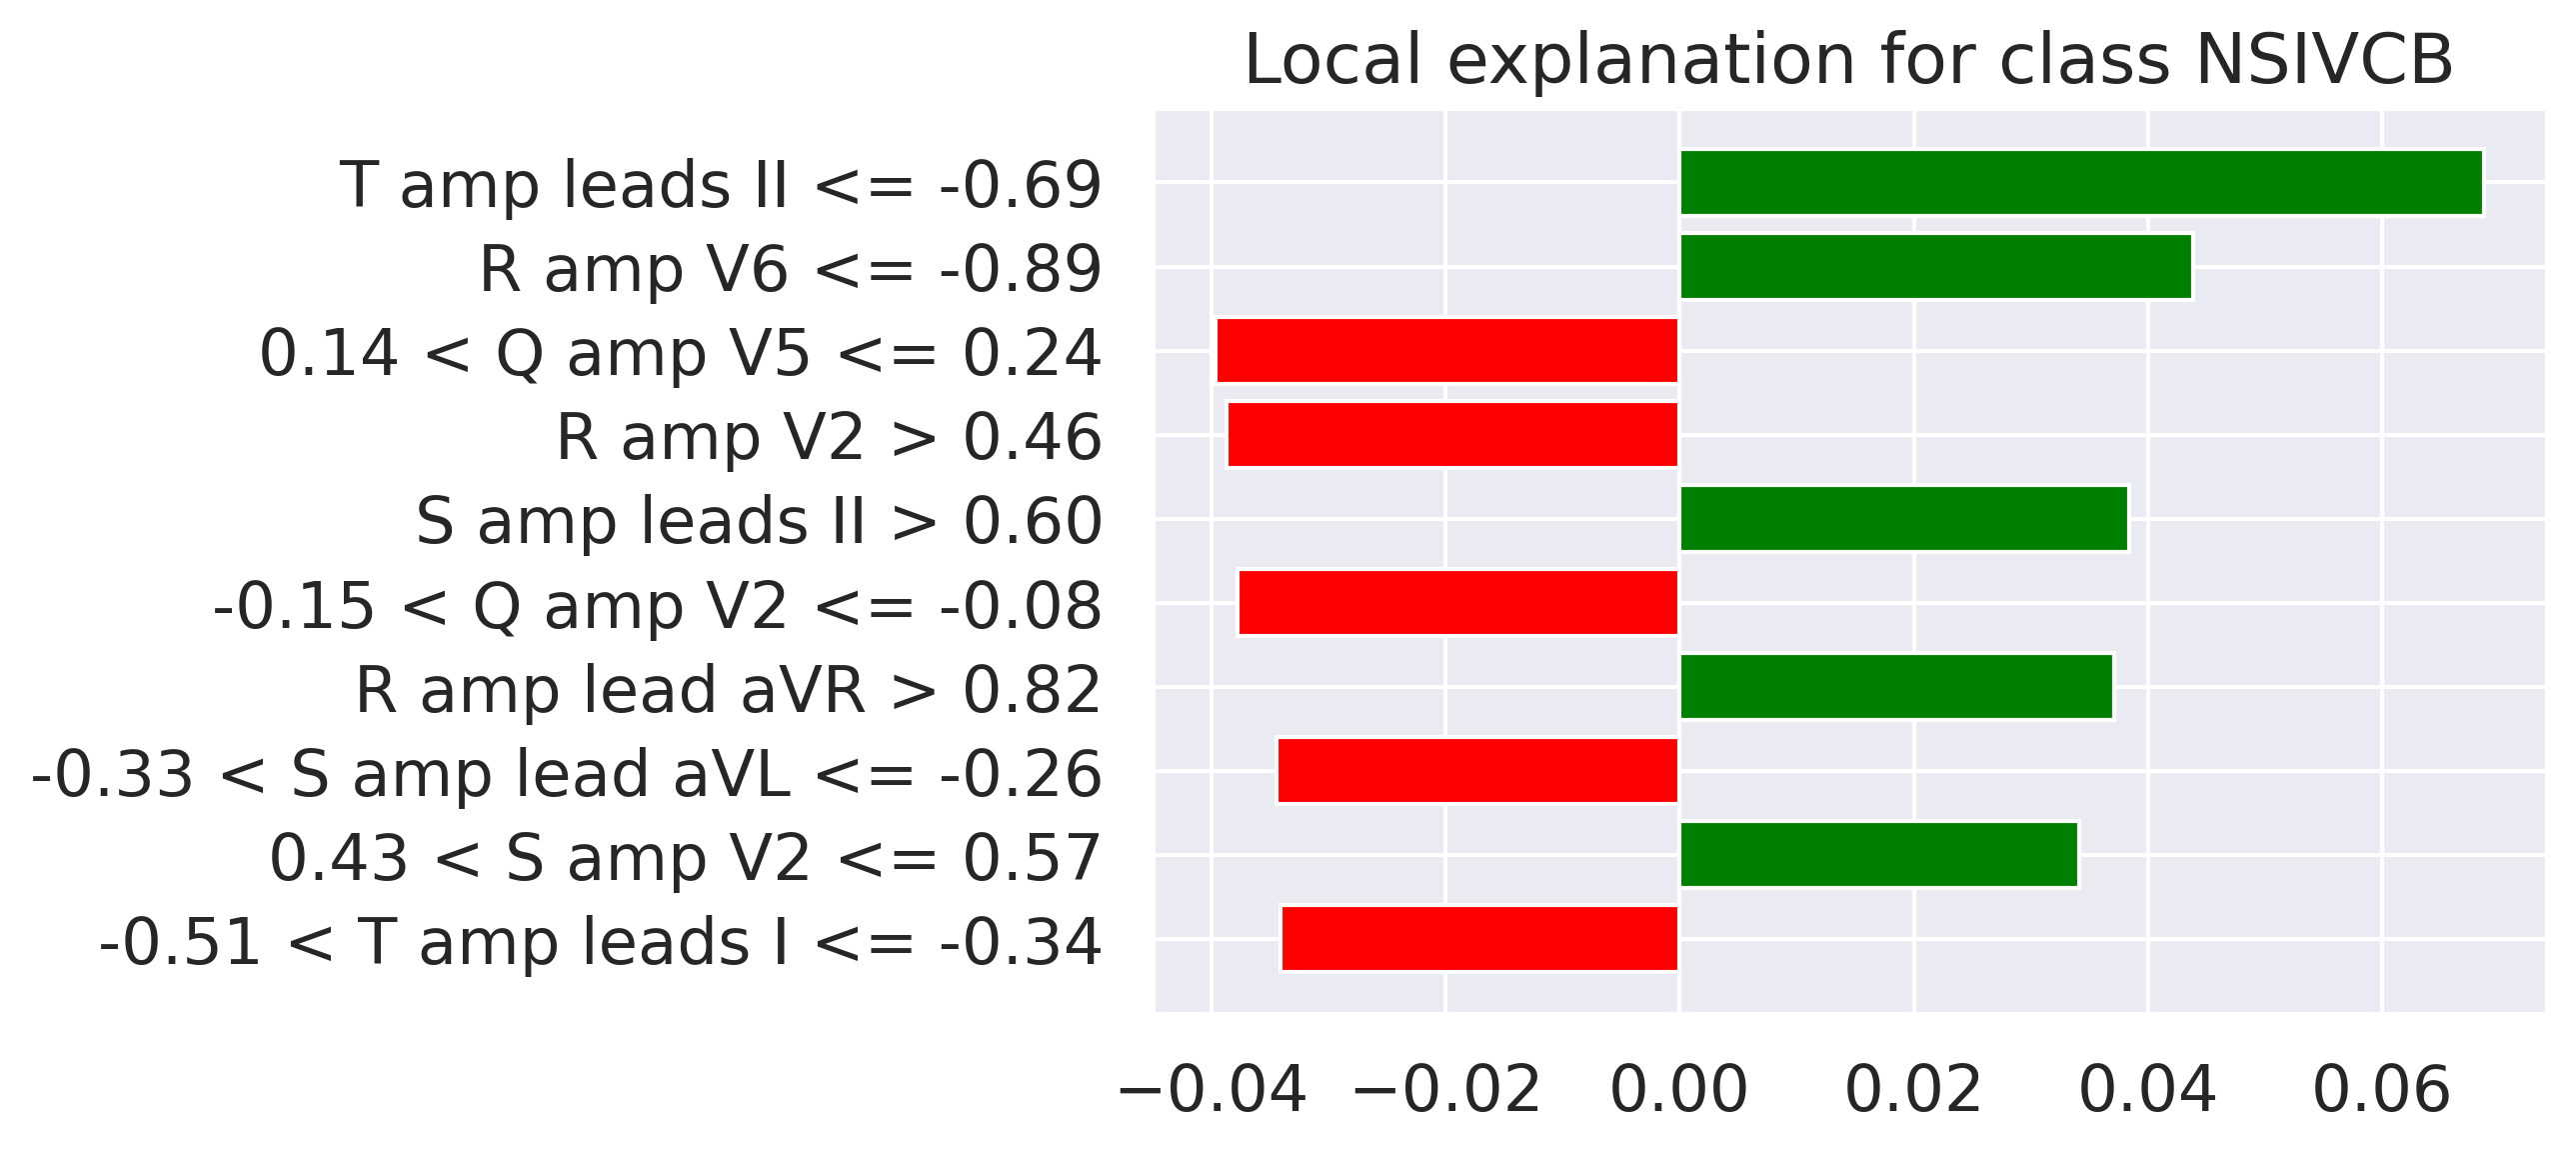
\includegraphics[width=.90\textwidth]{Figures/conduction_disorder_12lead.png}
    \caption{The figure shows the top $10$ features from a ECG that contributed with the prediction. In the labels on the vertical axis; amp is short for amplitude, P, Q, R,S,T are the characteristic peaks in the ECG and $I$, $II$, $III$, aVL, aVF, aVR, V1, V2, V3, V4, V5 and V& are the name of the 12 ECG leads. The ECG-features are extracted from a ECG from a patient with non-specific intra ventricular conduction disorder (NSIVCB).  The green bars indicate the the degree of contribution towards an positive classification of NSIVCB, while the red bars shows the degree of contribution towards a negative classification of NSIVCB.}
    \label{fig:explainability_rand_12}
\end{figure}
%\begin{figure}[!bp]
%    \centering
%    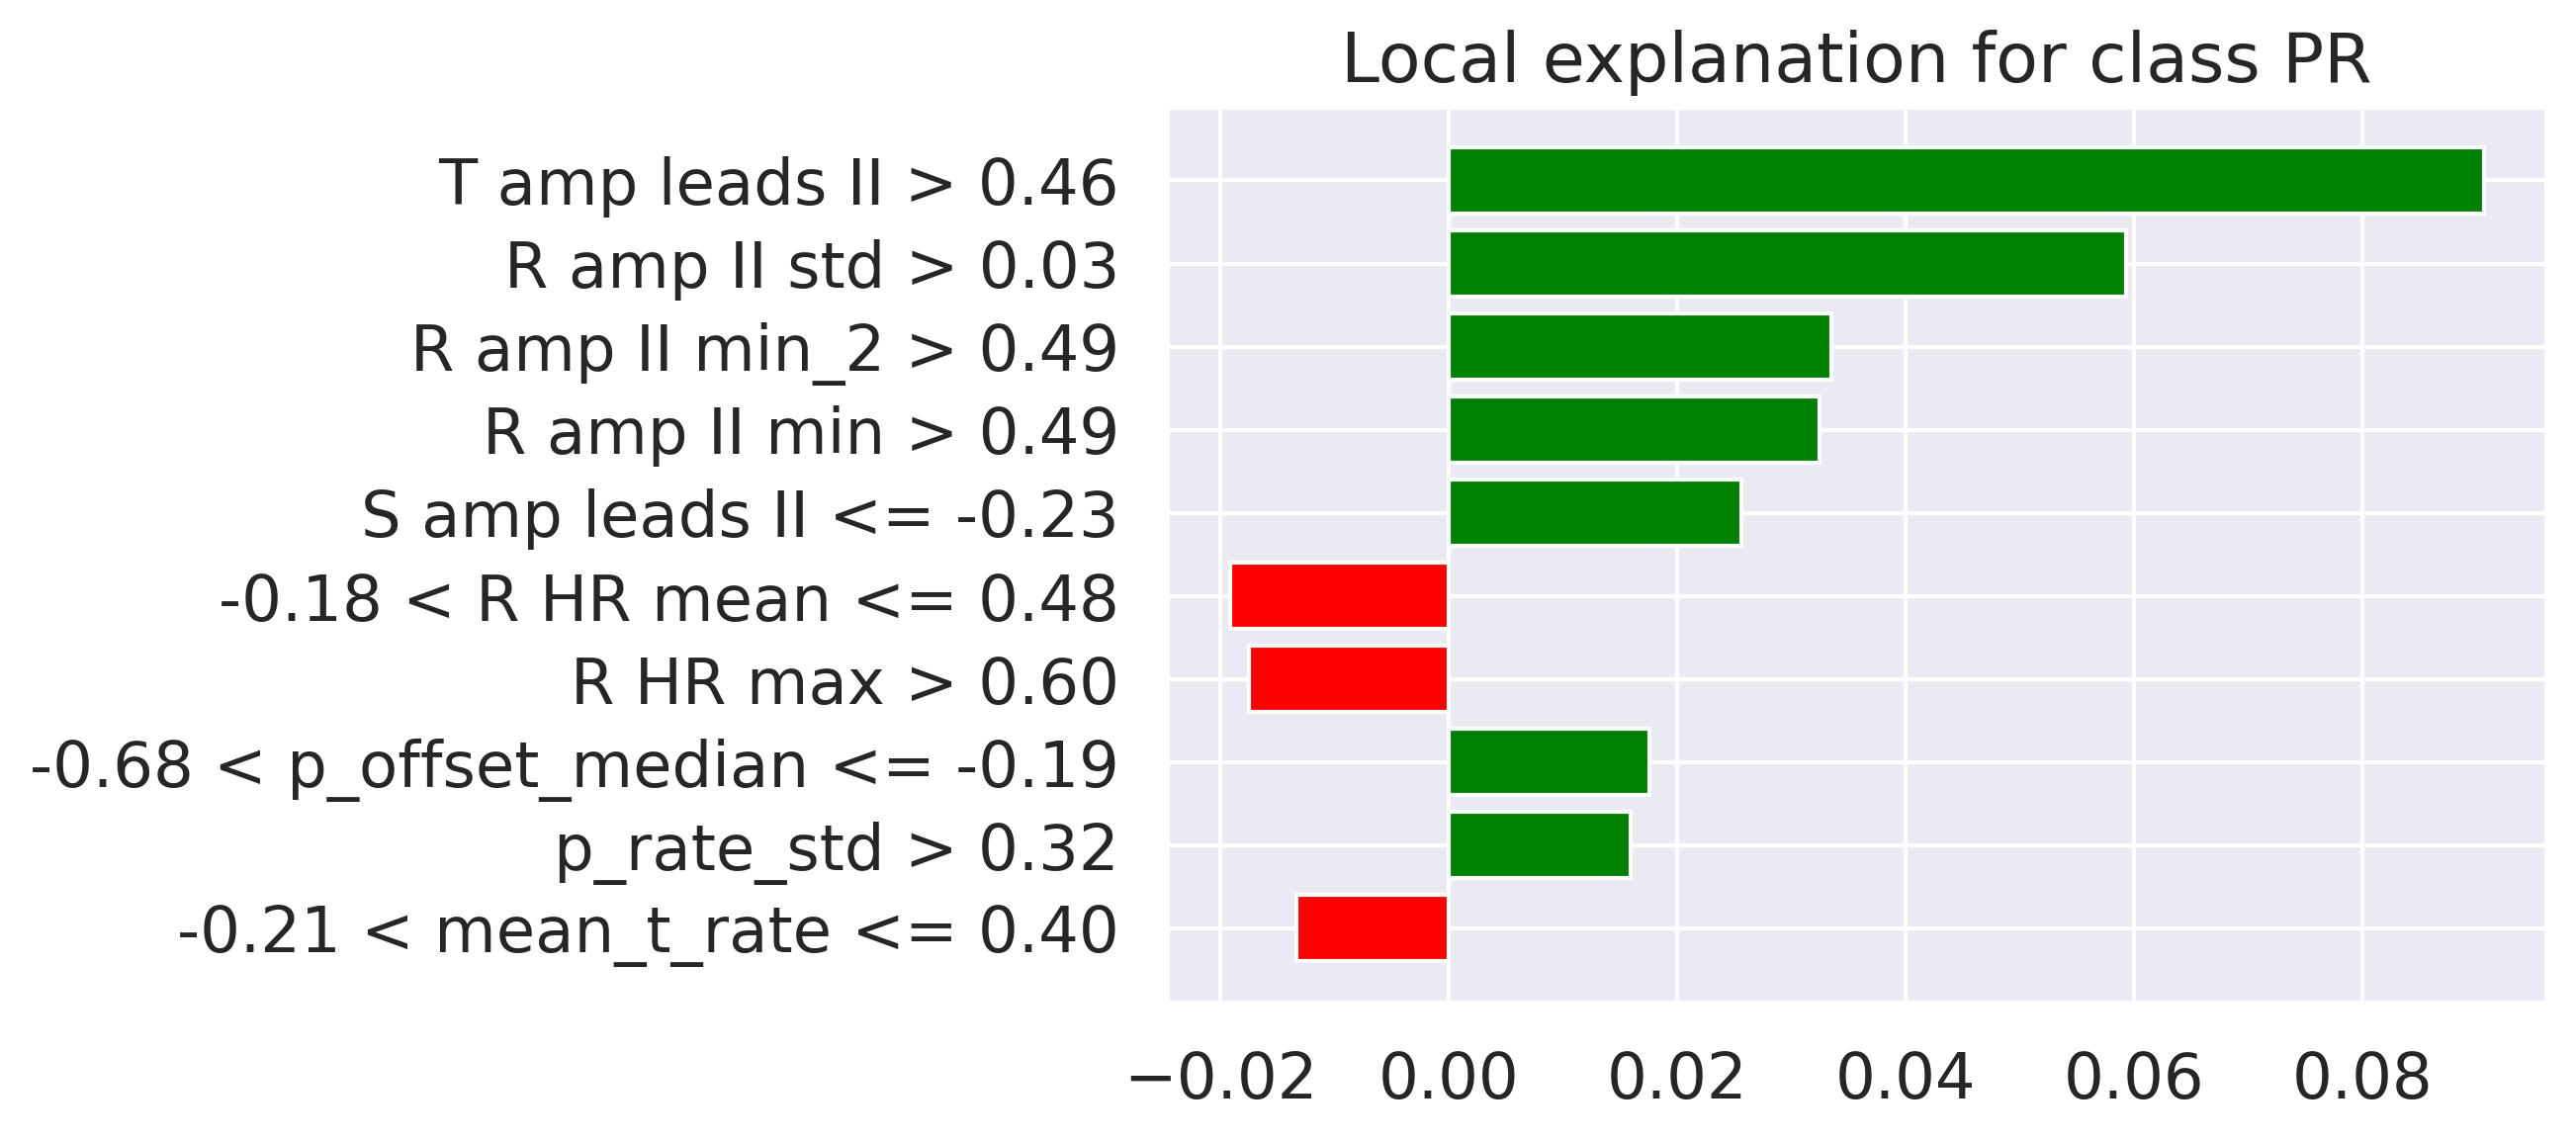
\includegraphics[width=1\textwidth]{Figures/pacing_rytm_2lead.png}
%    \caption{}
%    \label{fig:parameterregel}
%\end{figure}
%\begin{figure}[!bp]
%    \centering
%    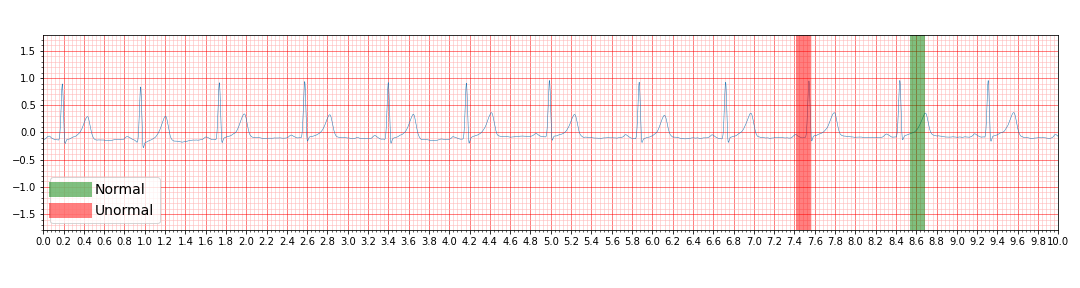
\includegraphics[width=1\textwidth]{Figures/Normal-V6.png}
%    \caption{The figure shows the explainability results from the Encoder 1D convolutional model. Sub-figure shows a 10 second ECG sequence of a normal ECG extracted from lead $II$ and sub-figure b show The vertical, transparent red bars in the plots indicate sections of the ECG that}
%    \label{fig:parameterregel}
%\end{figure}

The recurrent explainer, used on the Encoder model, was trained on $5000$ ECGs from the training data and then tested on a ECG from the test data. the ECG from the test data were abnormal and predicted correctly by the CNN model. The explaination model returned the channel/lead and the index of the sample/feature that were most important for the prediction by the Encoder. Figure \ref{fig:expl_cnn} shows the tree most important features in lead aVR for the given test data.

\begin{figure}[!htp]
    \centering
    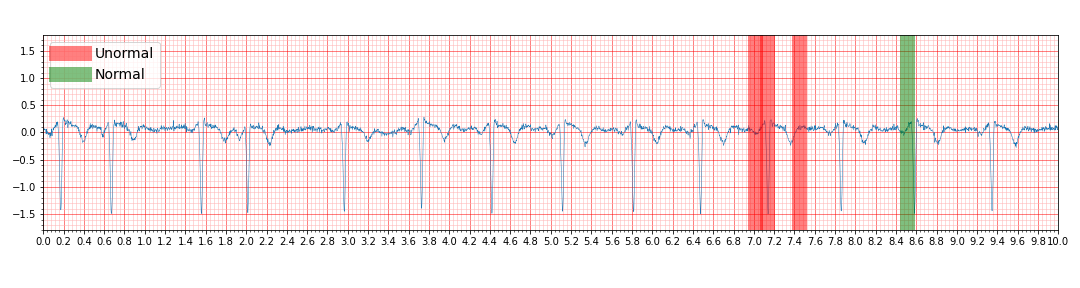
\includegraphics[width=1\textwidth]{Figures/Abnormal-aVR.png}
    \caption{The figure shows a 10 seconds long ECG-recording from the aVR-lead. The ECG is correctly classified as abnormal by a 1D CNN Encoder. The horizontal, transparent green and red lines marks the features in the ECG that is seen as normal and abnormal by the recurrent explaination model. THe green line indicates the parts of the ECG that contributes towards a normal classification while the red line indicates the parts the ECG that contributes towards an abnormal classification.}
    \label{fig:expl_cnn}
\end{figure}

\newpage



\section{Discussion}

This paper demonstrates how CNN and ensemble models can be used to classify multiple cardiac abnormalities using 12-lead ECG-recordings. The cross-validated results show that the ensemble model, using features from 12 leads, outperforms the other nine models on the development dataset from PhysioNet/CinC Challenge 2020. F1, F2, G2 and the PhysioNet/CinC Challenge Score were used to score the models. The 12-lead ensemble model was significantly better than all other models, measured on all four metrics.

The winner of PhysioNet/CinC Challenge 2020 reported a mean  cross-validated PhysioNet/CinC Challenge Score of $0.533\pm0.046$ SD \cite{natarajan_wide_nodate}, which was slightly better than the best score achieved in this study: $0.512\pm 0.006$. It is important to bear in mind that the cross-validated scores achieved on the development set, in this study, should be compared with caution to the reported scores on the PhysioNet/CinC Challenge 2020 hidden test set from other studies \cite{natarajan_wide_nodate,singstad_convolutional_nodate}. Even if some papers demonstrated good agreement between their cross-validated results, on the development set, and the results achieved on the hidden test set \cite{natarajan_wide_nodate}, the organizer reported that high-performing algorithms exhibited significant drops ($\approx 10\%$) in performance on the hidden test data \cite{alday_classification_2020}.

Surprisingly, the CNNs with the lowest complexity performed best compared to the rest of the CNNs. The Encoder model was significantly better in terms of F1, F2 and G2-score (figure \ref{fig:crossval_score}a-c), but closely followed by FCN and FCN $||$ Gender\&Age when looking at the PhysioNet/CinC Challenge Score (Figure \ref{fig:crossval_score}d). Nevertheless, it is stated in \cite{singstad_convolutional_nodate} that the Encoder performed worse than FCN $||$ Gender\&Age, Encoder $||$ Gender\&Age, Encoder $||$ FCN + rule-based model and Encoder $||$ FCN $||$ Gender\&Age + rule-based model on a subset of the hidden test set. This observation emphasizes that one should be careful when comparing cross-validated scores with scores achieved on the hidden test set.

The FCN $||$ Encoder and the FCN $||$ Encoder $||$ Gender\&Age appeared to be unaffected by adding the rule-based model. No significant differences can be seen for any of the scoring methods in figure \ref{fig:crossval_score}. A possible explanation for this might be that the rule-based model always agreed with the CNN-model and thus did not change the prediction. Another possible explanation for this is that the rule-based algorithms failed to analyze the ECG and then did not make any prediction. One should keep in mind that these rule-based algorithms were really simple and therefore these results should be interpreted with caution.

Another surprising aspect was that the ensemble model, using features from 2 leads, performed significantly better than all CNN models, using all 12 leads, on the PhysioNet Challenge Score (figure \ref{fig:crossval_score}d). However, it should be mentioned that the Encoder performed equally well on the F1, F2 and G2-score as seen in figure \ref{fig:crossval_score}a-c.

A possible limitation in this study is that the ECGs were not filtered before feeding them into the model or before extracting features with the ECG-featurizer. Some of the ECGs had a lot of noise, like the ECG in figure \ref{fig:noisy_leadII}. Further studies are needed to determine if a filtered ECG signal would improve the performance of the models used in this study.

\begin{figure}[!hbp]
    \centering
    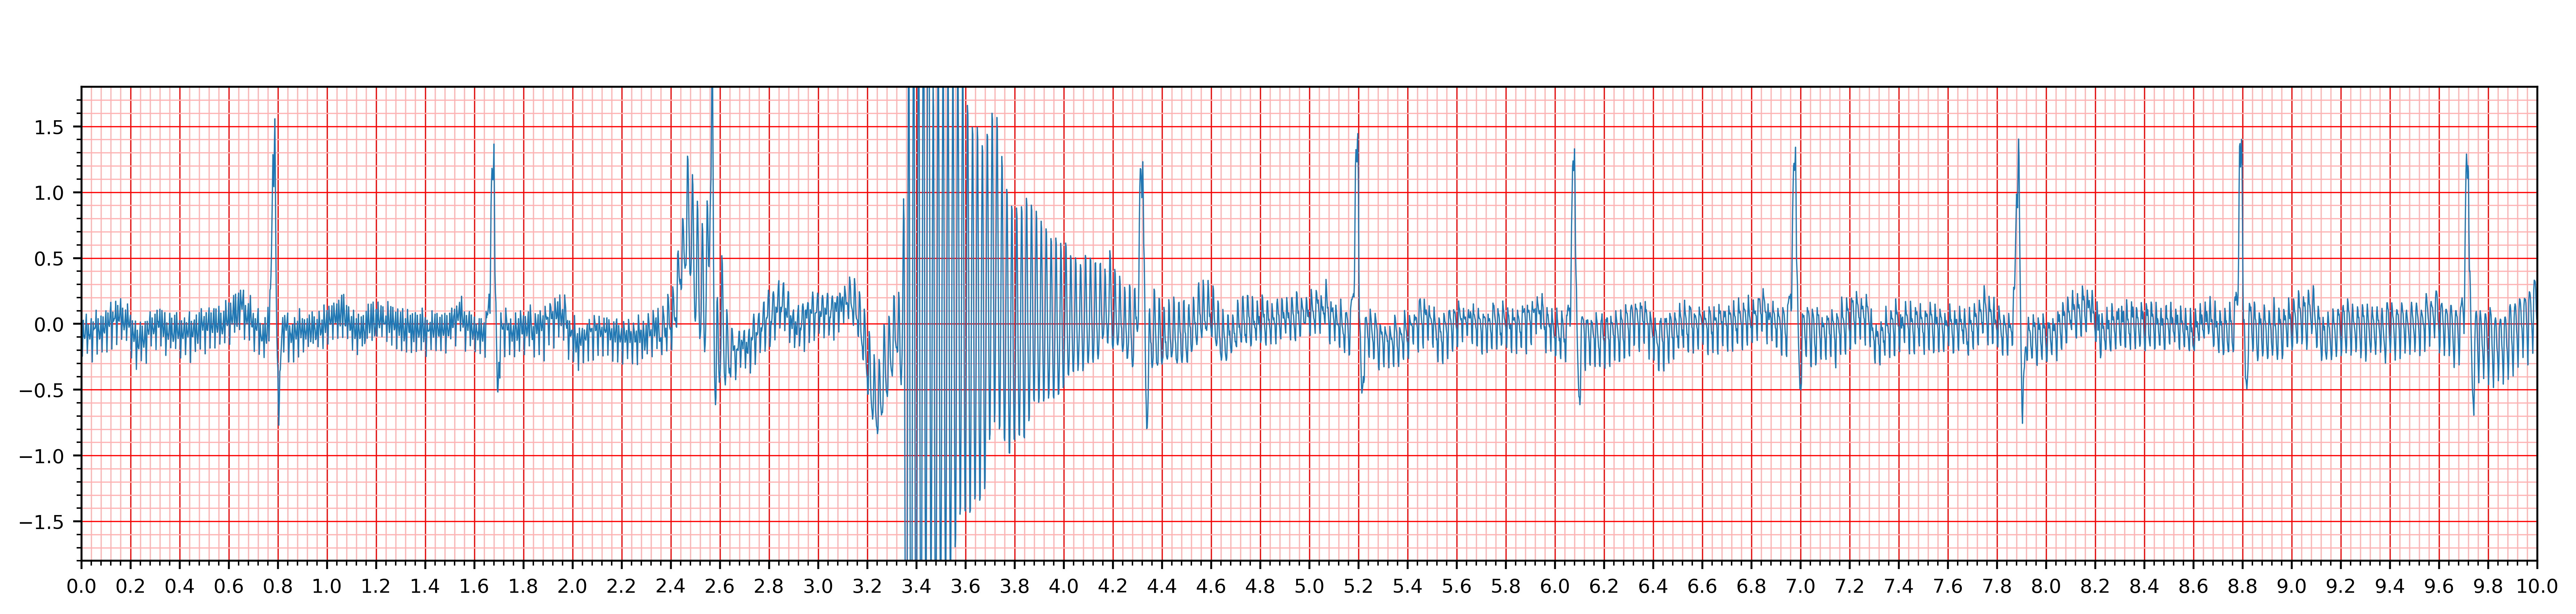
\includegraphics[width=.90\textwidth]{Figures/noisy_leadII.png}
    \caption{The figure shows an example, from the development set, of a noisy ECG-signal from lead II}
    \label{fig:noisy_leadII}
\end{figure}

This research has demonstrated two slightly different methods of using explainable AI with ECG classifiers. The prediction made by the ensemble model is based on the extracted ECG features using the ECG-featurizer and therefore the explanation, by LIME, are related and limited to these features. On the other hand, the prediction made by the CNN models is based on $12 \times 5000$ samples giving LIME more features to use in its explanation.




Even if the ensemble model only used a few features ($112$) compared to the CNN models ($12 \times 5000$), the explanation provided for the ensemble model seems to be more understandable in this case. In figure \ref{fig:explainability_rand_12} the most important explanation for the AF prediction  was the standard deviation of the heart rate calculated from the R-peaks. This explanation can be supported by physiological knowledge.

The explanation of the ECG time series has shown to have some potential \cite{strodthoff_deep_2020,zhang_interpretable_2020}. However, in this study, there is hard to see any patterns from the three segments highlighted by the recurrent explainer in figure \ref{fig:expl_cnn}. In future research, the recurrent  explainer should be programmed to return more of the features that were used in the prediction to see any patterns.

A general limitation with LIME is that it is built on a weak mathematical foundation compared to for example the SHAP library \cite{lundberg_unified_2017} (Shapley values). 
In future investigations, it should be considered to use a different approach like the SHAP library to explain the predictions of the classifiers. 


Despite the results showing that explainable AI methods can be used to explain the classification of ECGs, there is still a lot of work to be done in this field. It is important to make sure that the explanations are valuable for potential end-users (doctors/cardiologists). In future investigations, it also might be possible for the developer to use the explanation to identify possible weaknesses of the classification model by looking at the explanations. Our findings emphasize the need to continue to develop explainable models for time series classifiers like the ECG models demonstrated in this study. 

\section{Conclusions}
The aim of the present research was to compare ten models and their feasibility to classify 12-lead ECGs with a large number of different diagnoses from multiple sources around the world. The findings reported, shed new light on the results reported in \cite{singstad_convolutional_nodate} by scoring all models using 10-folded cross-validation. In addition, two new ensemble models were developed. The one that used ECG features from all 12 leads outperformed all other models in this study. Also, the ensemble model, using only features from 2 leads, showed promising results compared to the 12-lead models. Although this study focuses mainly on 12-lead ECG, these findings may well have a bearing on Holter-ECG which normally utilizes one or two leads.

The second aim of this study was to investigate the usefulness of LIME for explaining the prediction from a CNN model and an ensemble model. The results of this investigation showed two different ways of explaining the prediction by the ECG classifiers. Despite of its limitations, the study certainly adds to our understanding of how explainable AI can be used for ECG classification. A new study with a greater focus on explainability could produce findings that may be of interest to doctors and cardiologists.

%\section*{Acknowledgments} 
%This is where you acknowledge contributors that are not authors. Someone may have provided you thoughts and data samples and didn't feel they had contributed enough. Any individuals you name must be contacted to check that they don't think they should be authors, and to approve you naming them. This is not true of organizations, such as funding bodies. However, they will have specific language to include. Check with them. Make sure you identify any funding sources. This is important for public access mandates and intellectual property, as well as for reporting to the sponsors. Note that identifying sponsors here will create a permanent link, that will carry with it some specific responsibilities and funding flows for IP. So don't just throw in everyone who funds you. Be appropriate. Here's an example in italics (but don't italicize):

{\it
The authors wish to acknowledge the support of the National Science Foundation Award 1636933, National Institutes of Health (Grant R01HL136205). Any opinions, findings, and conclusions or recommendations expressed in this material are those of the author(s) and do not necessarily reflect the views of the National Science Foundation or the National Institutes of Health.

CL was funded by the International Post-doctoral Exchange Programme of the National Postdoctoral Management Committee of China and Emory University. We also would like to thank Arvind Ananthan and MathWorks, for their valuable assistance, free licenses to competitors and financial support of the Challenge.  Finally, we thank all the Challenge competitors themselves, without whom there would be no competition. } 

You must acquire the approval of anyone you acknowledge. You can't just thank people for advice or helping without asking them, because it may imply they approve of your work.
In this example, only the named person needs to be contacted for approval because they represent the company that is mentioned (MathWorks). If naming a company, it is important to check with a representative of the company to avoid any friction. They may not want to be associated with your article.


\def\newblock{\hskip .11em plus .33em minus .07em}

%\bibliographystyle{dcu}
\bibliographystyle{naturemag}
\bibliography{references}



%-------------------

\newpage
\appendix
\addcontentsline{toc}{chapter}{Appendix}
%is the aim of this years challenge to be able to classify diagnoses both from 2 and 12 lead ECG. This can give benefit for methods such as Holter-ECG and not only the clinically used 12-lead ECG. 
\newline\indent This study aims to develop an algorithm for automatic identification of cardiac abnormalities based on “The China Physiological Signal Challenge 2018”, containing 6877 12-lead ECG recordings, sampled at 500 Hz with a length between 6 and 60 seconds and labeled with 9 classes.


Automated ECG interpretation can assist health personnel in diagnosing ECGs. Current clinically used ECG use rule based algorithms which seems to be poor at detecting arrythmias, conduction disorders and pace maker rythms. On the other hand, modern artificial intelligence (AI) methods have proven to be superior in many fields. In the field of ECG interpretation, it has proven to work generally well in classifying arrhythmias, but there is still a lot work to be done in the field of using AI on all sorts of heart related pathology.
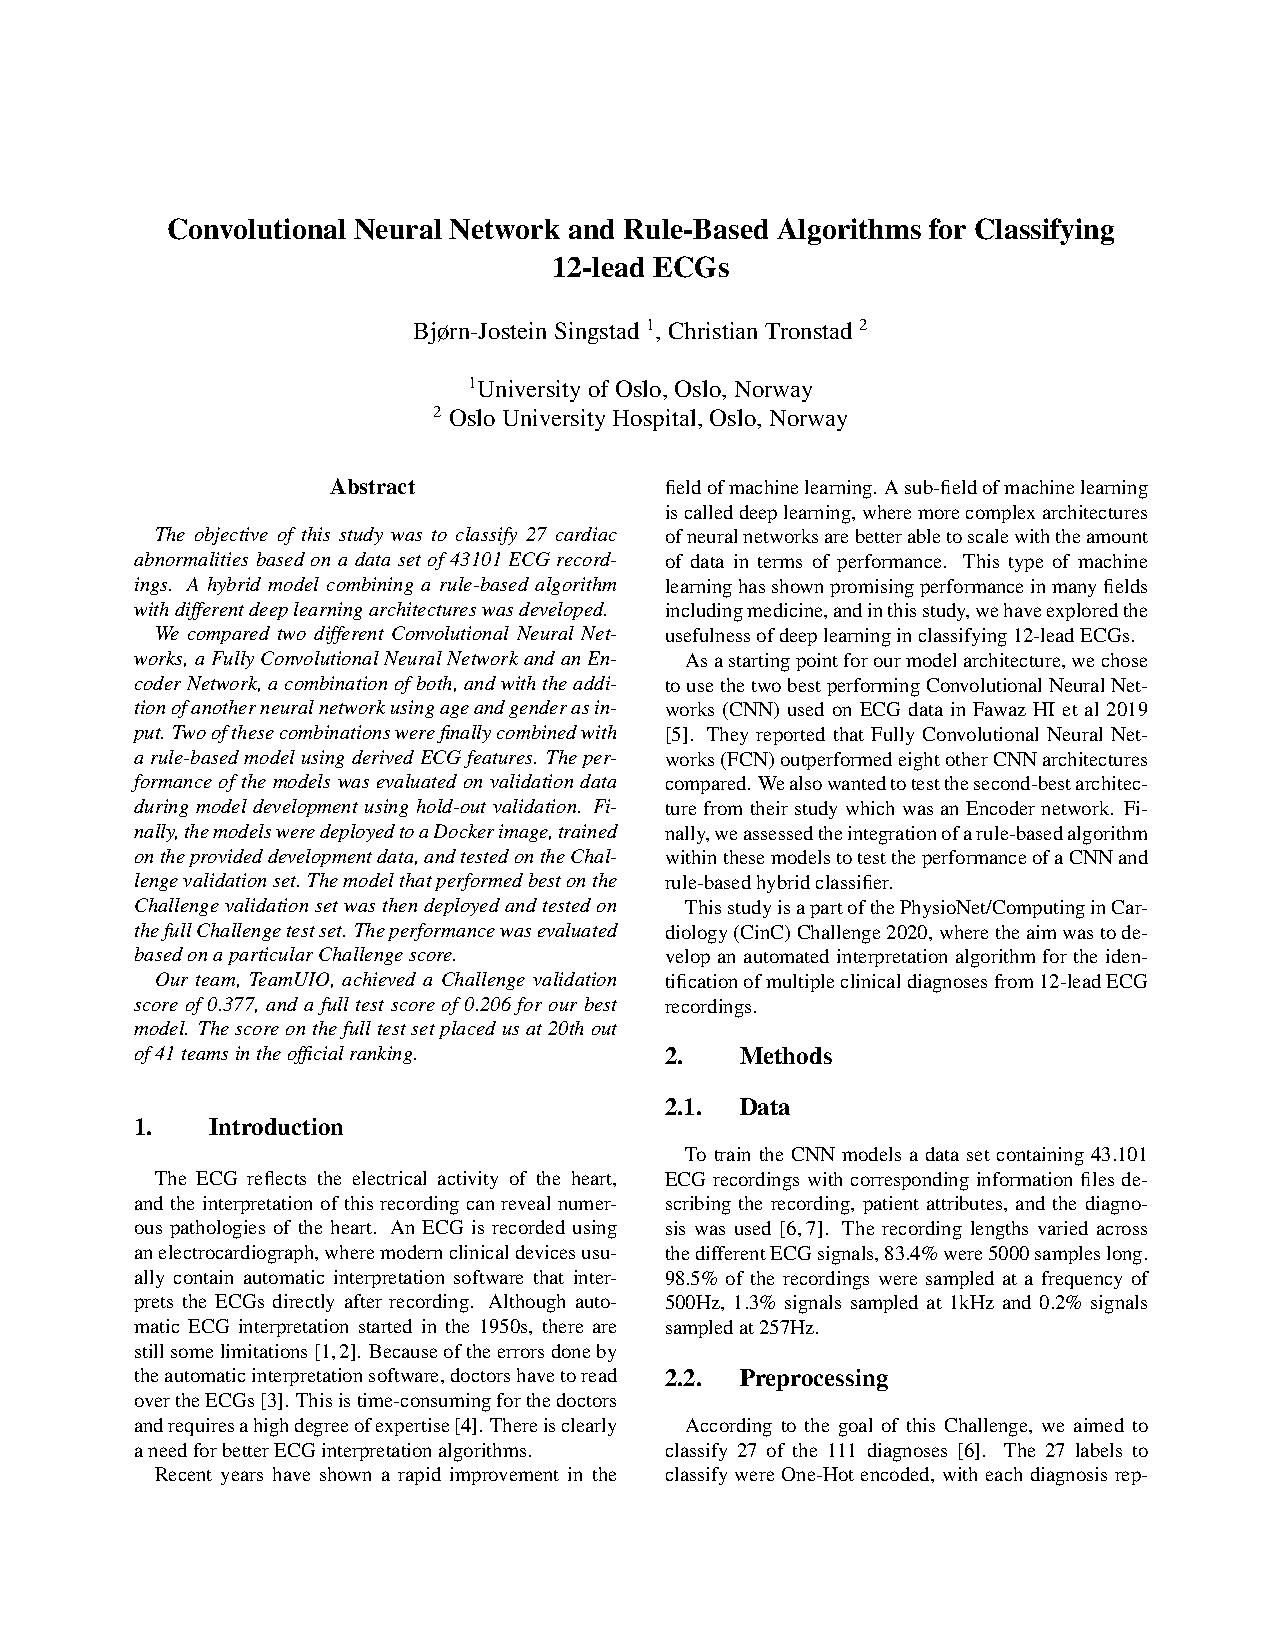
\includepdf[pages=-]{227.pdf}

\end{document}